% !TEX program = pdflatex
% !TEX enableSynctex = true
% !BIB program = bibtex

\documentclass[12pt]{article}

\usepackage{setspace}
\usepackage{amsmath}
\usepackage{amsfonts}
\usepackage{graphicx}
\usepackage{float}
\usepackage{dsfont}
\usepackage{natbib}
\addtolength{\oddsidemargin}{-.7in}
\addtolength{\evensidemargin}{-.7in}
\addtolength{\textwidth}{1.4in}
\usepackage{enumerate}
\onehalfspacing
\usepackage{geometry} % Required for customizing page layout
\usepackage{ragged2e}

\usepackage{caption}
\usepackage{booktabs}

\usepackage{hyperref}
\hypersetup{
	pdfstartview = FitH,
	pdfauthor = {...},
	pdftitle = {...},
	pdfkeywords = {...; ...; ...; ...},
	colorlinks = true,
	linkcolor = blue,
	urlcolor = blue,
	citecolor = blue,
	linktocpage=true
}

\DeclareMathOperator{\E}{\mathbb{E}}
\DeclareMathOperator*{\argmax}{arg\,max}
\DeclareMathOperator*{\argmin}{arg\,min}

\title{Corporate credit frictions under heterogeneous debt contracts}
\date{}

\begin{document}

\author{Barnabás Székely}
\date{\today}
\vspace{-1in}

\maketitle

\begin{abstract}
\noindent

Corporate credit market frictions are traditionally viewed as asset-based borrowing constraints. On the other hand, recent contributions argue that most of corporate debt is backed by cash-flows, which implies the prevalence of earnings-based borrowing constraints. Neither approach is entirely accurate. I find that most North American listed companies hold heterogeneous portfolio of debt contracts, which subjects them combination of asset-based and earnings-based frictions simultaneously. This paper explores the nature of corporate credit market frictions along these lines. First, it considers firms' optimal debt financing strategies. Cash flow-backed lending allows lenders to extract borrowers' going-concern value, which might yield more lenient credit conditions. However, as the empirical analysis suggests, this is subject to substantial fixed costs. These findings inform a structural heterogeneous agents model, which provides a formal description of corporate credit frictions and their effect on the economy.

\bigskip{}
\bigskip{}
%\bigskip{}
%\bigskip{}
%\vspace{-0.5cm}

Keywords: Heterogeneous firms, Credit market frictions, Cash flow-based lending, Earnings-based constraints

\medskip{}
% JEL Classification Code: E32, C22, E27.
\end{abstract}
\thispagestyle{empty}

\pagebreak{}


\section{Introduction \label{sec:introduction}} 

Corporate credit market frictions are traditionally characterized in the macro-finance literature as asset-based borrowing constraints. Recent contributions challenged this perspective. These argue that the majority of corporate debt is backed by borrowers’ future cash flows rather than assets - hence, credit frictions are better described as borrowing constraints based on current earnings. Such results led to the re-evaluation of the role of credit frictions in macroeconomic models. However, these studies typically view asset-based and CF-based lending as mutually exclusive, competing models of reality. This reduces this debate to addressing which constraint is more relevant for a greater number of firms. \vspace{3mm} \\
I argue that categorizing firms strictly as either asset-based or cash flow-based borrowers does not describe their debt financing problem accurately. This is motivated by the observation that most North American, listed non-financial corporations hold heterogeneous portfolio of asset-based and cash flow-based debt contracts. Hence, accounting for asset-based and earnings-based frictions simultaneously would better describe firms' debt financing problem. \vspace{3mm} \\
Building on an empirical analysis of debt financing strategies, this paper explores the determinants the credit frictions experienced by non-financial corporations. Then, it implements these frictions in a heterogeneous agents, general equilibrium model. The purpose of this structural model is twofold. It provides an accurate description of the nature of credit constraints as a function of firms' optimal debt financing strategy. Second, it estimates the effects of these `hybrid' credit frictions on the overall economy. 
\vspace{3mm} \\
Section \ref{sec:quantitative analysis} deals with empirical analyses. First, it introduces the data and discusses the classifications of credit contracts as asset or cash flow-based debt. I differentiate asset-based and cash flow-based debt contracts along the following principles:  
\begin{itemize}
\item \textit{asset-based lending} (ABL): secured against borrowers' (physical) assets and lenders expect in-default payments to be determined by the liquidation value or the collateral
\item \textit{cash flow-based lending} (CFL): no specific assets pledged as collateral and lenders expect in-default payments to be determined by the going-concern value or the firm.
\end{itemize}
Next, it studies the distribution of these debt contracts on the firm level. The main findings are the following: 52.1\% of firms hold asset-based and cash flow-based debt contracts simultaneously - these firms collectively account for 87.3\% of total asset value in the sample. Moreover, 36\% of firms rely only on asset-based financing. These firms are significantly smaller and less indebted, which implies that lending against future cash flows is subject to substantial fixed costs. Finally, I find that other than size (measured by assets), leverage and the share of collateralizable assets on the balance sheet (asset pledgeability) are important determinants of the reliance on CF-based borrowing. \vspace{3mm} \\
Section \ref{sec: qualitative analysis} carries out a qualitative analysis of the US bankruptcy code and highlights some key principles that later inform the structural model.\footnote{To enhance external validity, I also discuss EU bankruptcy codes in the appendix.} Furthermore, it identifies two potential sources of fixed costs of lending against future cash flows. First, CFL lending is based on the anticipation that the borrower will be reorganized should financial difficulties arise. Hence, the lender must take into account the potential legal, personnel and time expenses associated with this process. Second, cash flow-based contracts require the lender to monitor the borrower on an ongoing basis, which imposes significant expenses on the lender even in the normal course of operation. \vspace{3mm} \\
Section \ref{sec:model} consolidates these findings in a dynamic general equilibrium model, that incorporates heterogeneous borrowers (firms) and a competitive lender. To better understand how financial frictions are shaped, one must first consider lenders' costs and payoffs under each type of debt contract. Cash flow-based debt contracts provide the opportunity to capture the post-reorganization value of the firm. On the other hand, the empirical analysis suggests that lending against future cash flows is subject to substantial fixed costs, which limits availability for small firms. Moreover, since cash-flow based contracts are not backed by collateral, they are less efficient at retrieving in-default default payments when the borrower is liquidated. This trade-off is at the core of the debt financing problem of firms. \vspace{3mm} \\ 
Firms' optimal debt financing strategy, determines the extent to which they are subject to earnings based or asset based frictions. In the case of larger firms, fixed costs are not substantial and liquidation is unlikely. These firms find it optimal to borrow chiefly against future cash flows, meaning that the financial frictions experienced by them are primarily shaped by their going-concern value. On the other hand, smaller firms might be closed out of the CF-based lending market altogether, due to high fixed costs. These firms are largely subject to asset-based frictions.   \vspace{3mm} \\
\textbf{Background and literature review} \\
This paper contributes to the strand of macro-finance literature that studies the determinants and the implications of corporate credit market frictions in structural models. The most influential contributions to this literature, such as Kiyotaki and Moore (1997) and Bernanke, Gertler, and Gilchrist (1999) modelled credit frictions as borrowing constraints determined by the value of firms' capital (or net wealth). These asset-based borrowing constraints became a prevalent feature of models with imperfect credit markets.  \vspace{3mm} \\ 
Recent contributions challenged this perspective based on more granular analyses of corporate credit contracts. Lian and Ma (2021) finds that the majority of corporate debt are not secured by any specific assets, but rather backed by future cash flows. This implies that credit frictions would be better described as borrowing constraints determined by the earnings of borrowers (i.e. earnings-based constraints). A closely related branch of literature studies debt covenants. Drechsel (2023) finds that the majority of debt covenants limit debt in the function of current earnings rather than assets. This aligns closely with Lian and Ma's assertion that earnings based constraints are more relevant. \vspace{3mm} \\
Such results led researchers to re-evaluate the role of credit frictions in macroeconomic models. The most straightforward approach is replacing asset-based constraints with earnings-based constraints in a representative firm model. This has been shown to have substantial effects on the model's outcomes. For instance, Greenwald (2019) points out that earnings based constraints introduce a direct channel monetary policy transmission to corporate investments. Lian and Ma (2021) shows that this mitigates the acceleration mechanism driven by asset price feedback. Drechsel and Kim (2022) argues that facing earings based constraints, firms 'under-borrow' relative to the social optimum, This highlights the importance of considering the specific form of financial constraints in designing regulatory policies.  \vspace{3mm} \\
One notable shortcoming of representative firm models is their inability to produce both types of lending in equilibrium.\footnote{Since the representative firm cannot be subject to both binding constraints at the same time.} This often leads to an `either-or' approach to corporate borrowing, where asset-based and cash flow-based lending are treated as competing models of reality. This view persists even when heterogeneous firms are considered. Drechsel (2023) considers a model in which a certain (exogenous) proportion of firms face asset-based constraints while the remaining firms are subject by earnings-based constraints. He finds that investment shocks (that affect the price of capital countercyclically) have the opposite effect on borrowing behavior depending on the borrowing constraints in place. Öztürk (2022) studies a heterogeneous agents model in which firms exhibit differences in productivity and value of total asset. This setup allows him to explore the choice between asset based or cash flow based debt financing, but he does not consider cases when firms have access to both type of contract simultaneously. \vspace{3mm} \\ 
Moreover, I rely on the strand of heterogeneous firms literature, which dates back to Hopenhayn (1992). In particular, I extend the model framework introduced Khan and Thomas (2013) and Khan, Senga and Thomas (2017), where firms are heterogeneous in assets and productivity, own capital and may borrow or save. This framework gained traction in recent research across various applications. For instance, Ottonello and Winberry (2020) and Jeenas (2019) stress the importance of considering differences in firms' financial position when studying the effects of monetary policy shocks. Other contributions build on heterogeneous firms framework to research financing choices over the life cycle, (Kochen, 2022), study the optimal maturity structure (Jungherr and Schott, 2020) or estimate the effects of firms rescue policies under the Covid induced recession (Di Nola, Kaas and Wang, 2023). Also closely related to my paper is Corbae and D'Erasmo (2021), who allow firms to choose between liquidation and reorganization under bankruptcy - but they do not consider heterogeneity in debt contracts.  \vspace{3mm} \\
In a broader context, this paper connects to the misallocation literature initiated by Hsieh and Klenow (2009).\footnote{See Hopenhayn (2014) and Restuccia and Rogerson (2012) for extensive reviews of this subject.} It extends the discussion on the role of financial frictions in exacerbating capital misallocation - such as Midrigan and Xu (2014), Banerjee and Moll (2010), Buera Kaboski and Shin (2011). Furthermore, my model shares similarities with Corbae and D'Erasmo (2021) and Azariadis, Kaas and Wen (2016). These studies emphasize that the external finance premium faced by companies is influenced by creditors' forward-looking expectations regarding the likelihood of financial distress or how it will be resolved. 

\section{Empirical analysis of credit constraints \label{sec:quantitative analysis}}
\subsection{Descriptive statistics \label{sec:descriptive stats}}

I study a total of 180388 debt contracts held by 8974 non-financial corporations between 2010Q1 and 2023Q2. Debt-level data is collected from S\&P's Capital IQ, and firm-level data is collected from Compustat North America. In the main body of this study, I analyze listed corporations, headquartered in the United States or Canada. Table 1. summarizes some firm and debt-level statistics over the observed time period. Later, I connect Capital IQ and ORBIS datasets to expand the cross-country coverage. The details of this analysis can be found in the appendix. \vspace{3mm} \\ 
Let me first discuss certain limitations the analysis. Since Compustat is restricted to traded companies, SMEs are underrepresented in the sample. Only 22\% of firms in the sample fit the definition of SMEs (less than 250 employees and 50 millions USD of assets, or 38.5 million USD of revenue). Another limitation is that I only observe firms that hold at least one debt contract. Therefore, I do not study the borrowing decisions on the extensive margin. Overall the dataset is not representative to the entire population of firms, but it includes the largest ones and those with a high potential for significant future growth.  Therefore, this analysis remains relevant for both the current and future performance of the production sector in the economy.

\begin{table}[H] 
\centering
\resizebox{\textwidth}{!}{%
\begin{tabular}{l|rrrrrr}
\multicolumn{7}{l}{\textbf{Firm-Level Summary Statistics}} \\
\hline
 & \textbf{Mean} & \textbf{p10} & \textbf{p25} & \textbf{Median} & \textbf{p75} & \textbf{p90} \\
Total Assets (millions USD) & 4456.87 & 5.57 & 41.80 & 381.76 & 2136.15 & 8077.88 \\
Qtr. Revenue (millions USD) & 893.06 & 0.00 & 3.47 & 65.17 & 417.56 & 1572.02 \\
Employees (thousands) & 10.57 & 0.02 & 0.12 & 1.05 & 5.90 & 20.90 \\
Equity (millions USD) & 1605.24 & 1.82 & 10.76 & 134.77 & 756.16 & 2774.05 \\
Investment rate (\%) & 1.41 & 0.00 & 0.13 & 0.55 & 1.48 & 3.53 \\
Firm Age (years) & 41.62 & 8.00 & 15.00 & 28.00 & 53.00 & 101.00 \\
Asset growth rate (\%) & 2.41 & -10.48 & -3.60 & 0.21 & 4.19 & 13.78 \\
Total debt value (millions USD) & 1569.56 & 0.60 & 5.05 & 72.10 & 702.12 & 3028.15 \\
Leverage & 0.35 & 0.03 & 0.11 & 0.27 & 0.45 & 0.70 \\
Debt to collateral & 0.51 & 0.11 &  0.26 &  0.52 & 0.75 & 0.89 \\ 
Asset Pledgeability (\%) & 50.80 & 9.92 & 25.72 & 51.93 & 75.87 & 90.21 \\
Liquidity & 0.16 & 0.01 & 0.03 & 0.08 & 0.20 & 0.44 \\
\hline
\end{tabular}%
}
\caption{\small Summary Statistics - all firms in the sample between 2010Q1 and 2023Q2}
\label{tab:sumstat}
\end{table}

\subsection{Classification: asset-based and CF-based contracts \label{sec:classification}}
Cash flow-based lending doesn't require borrowers to offer specific physical collateral. Instead, these loans may be unsecured or secured against the entire corporate entity (substantially all assets) or equity. In the absence of tangible collateral, lenders' in-default payoffs are chiefly determined by the borrower's going-concern value. Hence, to assess the risk inherent to each debt contract, lenders must monitor borrowers’ cash flows and evaluate their prospects on an ongoing basis.  \vspace{3mm} \\
Asset-based debt, on the other hand, is secured against borrowers’ collateral. This allows lenders to recover in-default payments through the liquidation of borrowers' assets. Extracting in-default payments is significantly more expensive and time-consuming when there is no collateral in place. Additionally, collateral alleviates lenders’ monitoring burden, as it requires only periodic appraisal of the borrowers' assets - although lenders typically still require borrowers to meet certain liquidity requirements, asset-based contracts generally place less emphasis on profitability. \vspace{3mm} \\
To differentiate between ABL and CFL contracts empirically, I follow the classification strategy adopted by Lian and Ma (2021). I assess the precision of my classification by comparing aggregate outcomes of to their reported results. \vspace{3mm} \\
Debt contracts not secured against a particular physical asset are classified as cash flow-based. In line with this, debentures and unsecured debt are counted towards CF-based debt. Bonds and notes are typically unsecured or secured against future cash flows (by liens on corporate entity or equity - Lian and Ma, 2021), which means that these are also best classified as cash flow-based debt. The sole exception to this are mortgage bonds, which are backed by real estate, and thus fall under the category of asset-based securities.\footnote{Furthermore, I classify  as asset-based debt contracts that contain the following words in their description: `mortgage', `building', `real estate' `plant', `property' or `collateral'. And classify debt contracts as cash flow-based that contain the following words in their description: `lien', `term facility', `term loan', `syndicated', `tranche', `acquisition line' and `bridge loan'.} Finally, capitalized leases are also classified asset-based. This leaves debt contracts that are categorized as `term loans', `revolving credit' and `other borrowings' by Capital IQ. Depending on the specifics of the contract, these can be asset-based and cash flow-based debt as well. To remain conservative about the share of cash flow-based debt, I classify these instruments as asset-based, unless they are unsecured.  \vspace{3mm} \\
I find that $52.4\%$ of debt instruments can be classified cash flow-based. Since these debt contracts are often large in terms of value, they collectively constitute 75.5\% of the total debt by volume. This aligns well with the findings reported by Lian and Ma (2021) who put the volume of cash flow-based debt to $80\%$. Nevertheless, it should be noted that due to data limitations, my approach is likely to yield a cruder classification - the lower share of CF debt is also probably down to the combination of less information on debt contracts and a conservative classifying strategy. The CF-based debt remains relatively stable (fluctuating within the range of 71.8\% to 79.8\%). However, it declines significantly in the year 2019 and remains subdued until the end of the period - see figure \ref{chart:CFLshare} in the appendix. 

\subsection{Reliance on cash flow-based debt financing \label{sec:CFL reliance}}
Firms typically rely on multiple debt instruments simultaneously. Over the sample period, non-financial corporations hold an average of 5.21 debt contracts. Moreover, only a minority (19\%) of them holds just a single contract. Importantly, the majority of firms hold cash flow-based and asset-based debt at the same time.\footnote{Various types of financing may be sought for different purposes. For instance, a company may decide to finance its daily operation by an asset-based revolving credit facility while seeking cash flow-based financing for its long-term investments. I do not attempt to recreate this level of detail. My goal is to study the extent to which firms rely on CFL lending in their debt portfolio.}  To facilitate firm-level analysis, I define the reliance on cash flow-based borrowing as follows: 
$$ \text{CFL reliance}  = \text{CFL debt } / \text{ Total debt} $$
Table \ref{tab:shares} outlines this variable, indicating that 35.7\% of firms exclusively have asset-based debt, while 12.2\% solely depend on cash flow-based financing. The rest, 52.1\% of firms hold both type of debt contracts at the same time. Since these are often the largest firms, this corresponds to 87.3\% after weighing with total assets. This is in contradiction to earlier analyses, which classify firms into two non-intersecting groups of asset-based and cash flow-based borrowers, subject to asset-based or earnings-based frictions respectively. Financial frictions experienced by most firms are often shaped by cash flow-based and asset-based considerations simultaneously. \vspace{3mm} \\
\noindent It is also worth noting the substantial proportion of borrowers hold asset-based debt contracts only. To better understand the decision to borrow (lend) against future cash flows, I differentiate between firms that only hold asset-based debt (ABL firms) and those that have a positive proportion of debt in their portfolio tied to their cash flows. Table \ref{tab:t-tests} in the appendix shows that asset-based borrowers are significantly smaller, younger and less indebted than CFL firms. This evidence is consistent with high fixed costs of borrowing (lending) against future cash flows. Section \ref{sec:fixed costs} discusses the potential sources of these fixed costs.  Moreover, figure \ref{chart:ridges} in the appendix shows the distribution of all three classes of borrowers.

\begin{table}[h!]
    \centering
    \begin{tabular}{l|rrr}
    \multicolumn{4}{l}{\textbf{Firm shares by debt financing strategy}} \\
    \hline
    \hspace{2.2cm} \textbf{Share by} & \textbf{\# of Firms} & \textbf{Assets}  & \textbf{Borrowing} \\  
    Asset-based borrowers & 35.66 \% & 4.83 \% & 3.36 \% \\ 
    `Hybrid' borrowers & 52.11 \% & 87.27 \% & 90.31  \% \\ 
    CF-based borrowers & 12.23 \% & 7.91 \% & 6.33  \% \\ 
       \bottomrule
    \end{tabular}
    \caption{\small Share of firms categorized by CF-reliance} 
    \label{tab:shares}
    \end{table}

\begin{figure}[H]  % [h] indicates placing the image here
    \centering
    \caption{The distribution of CFL reliance} \label{chart:CFLcdf}
    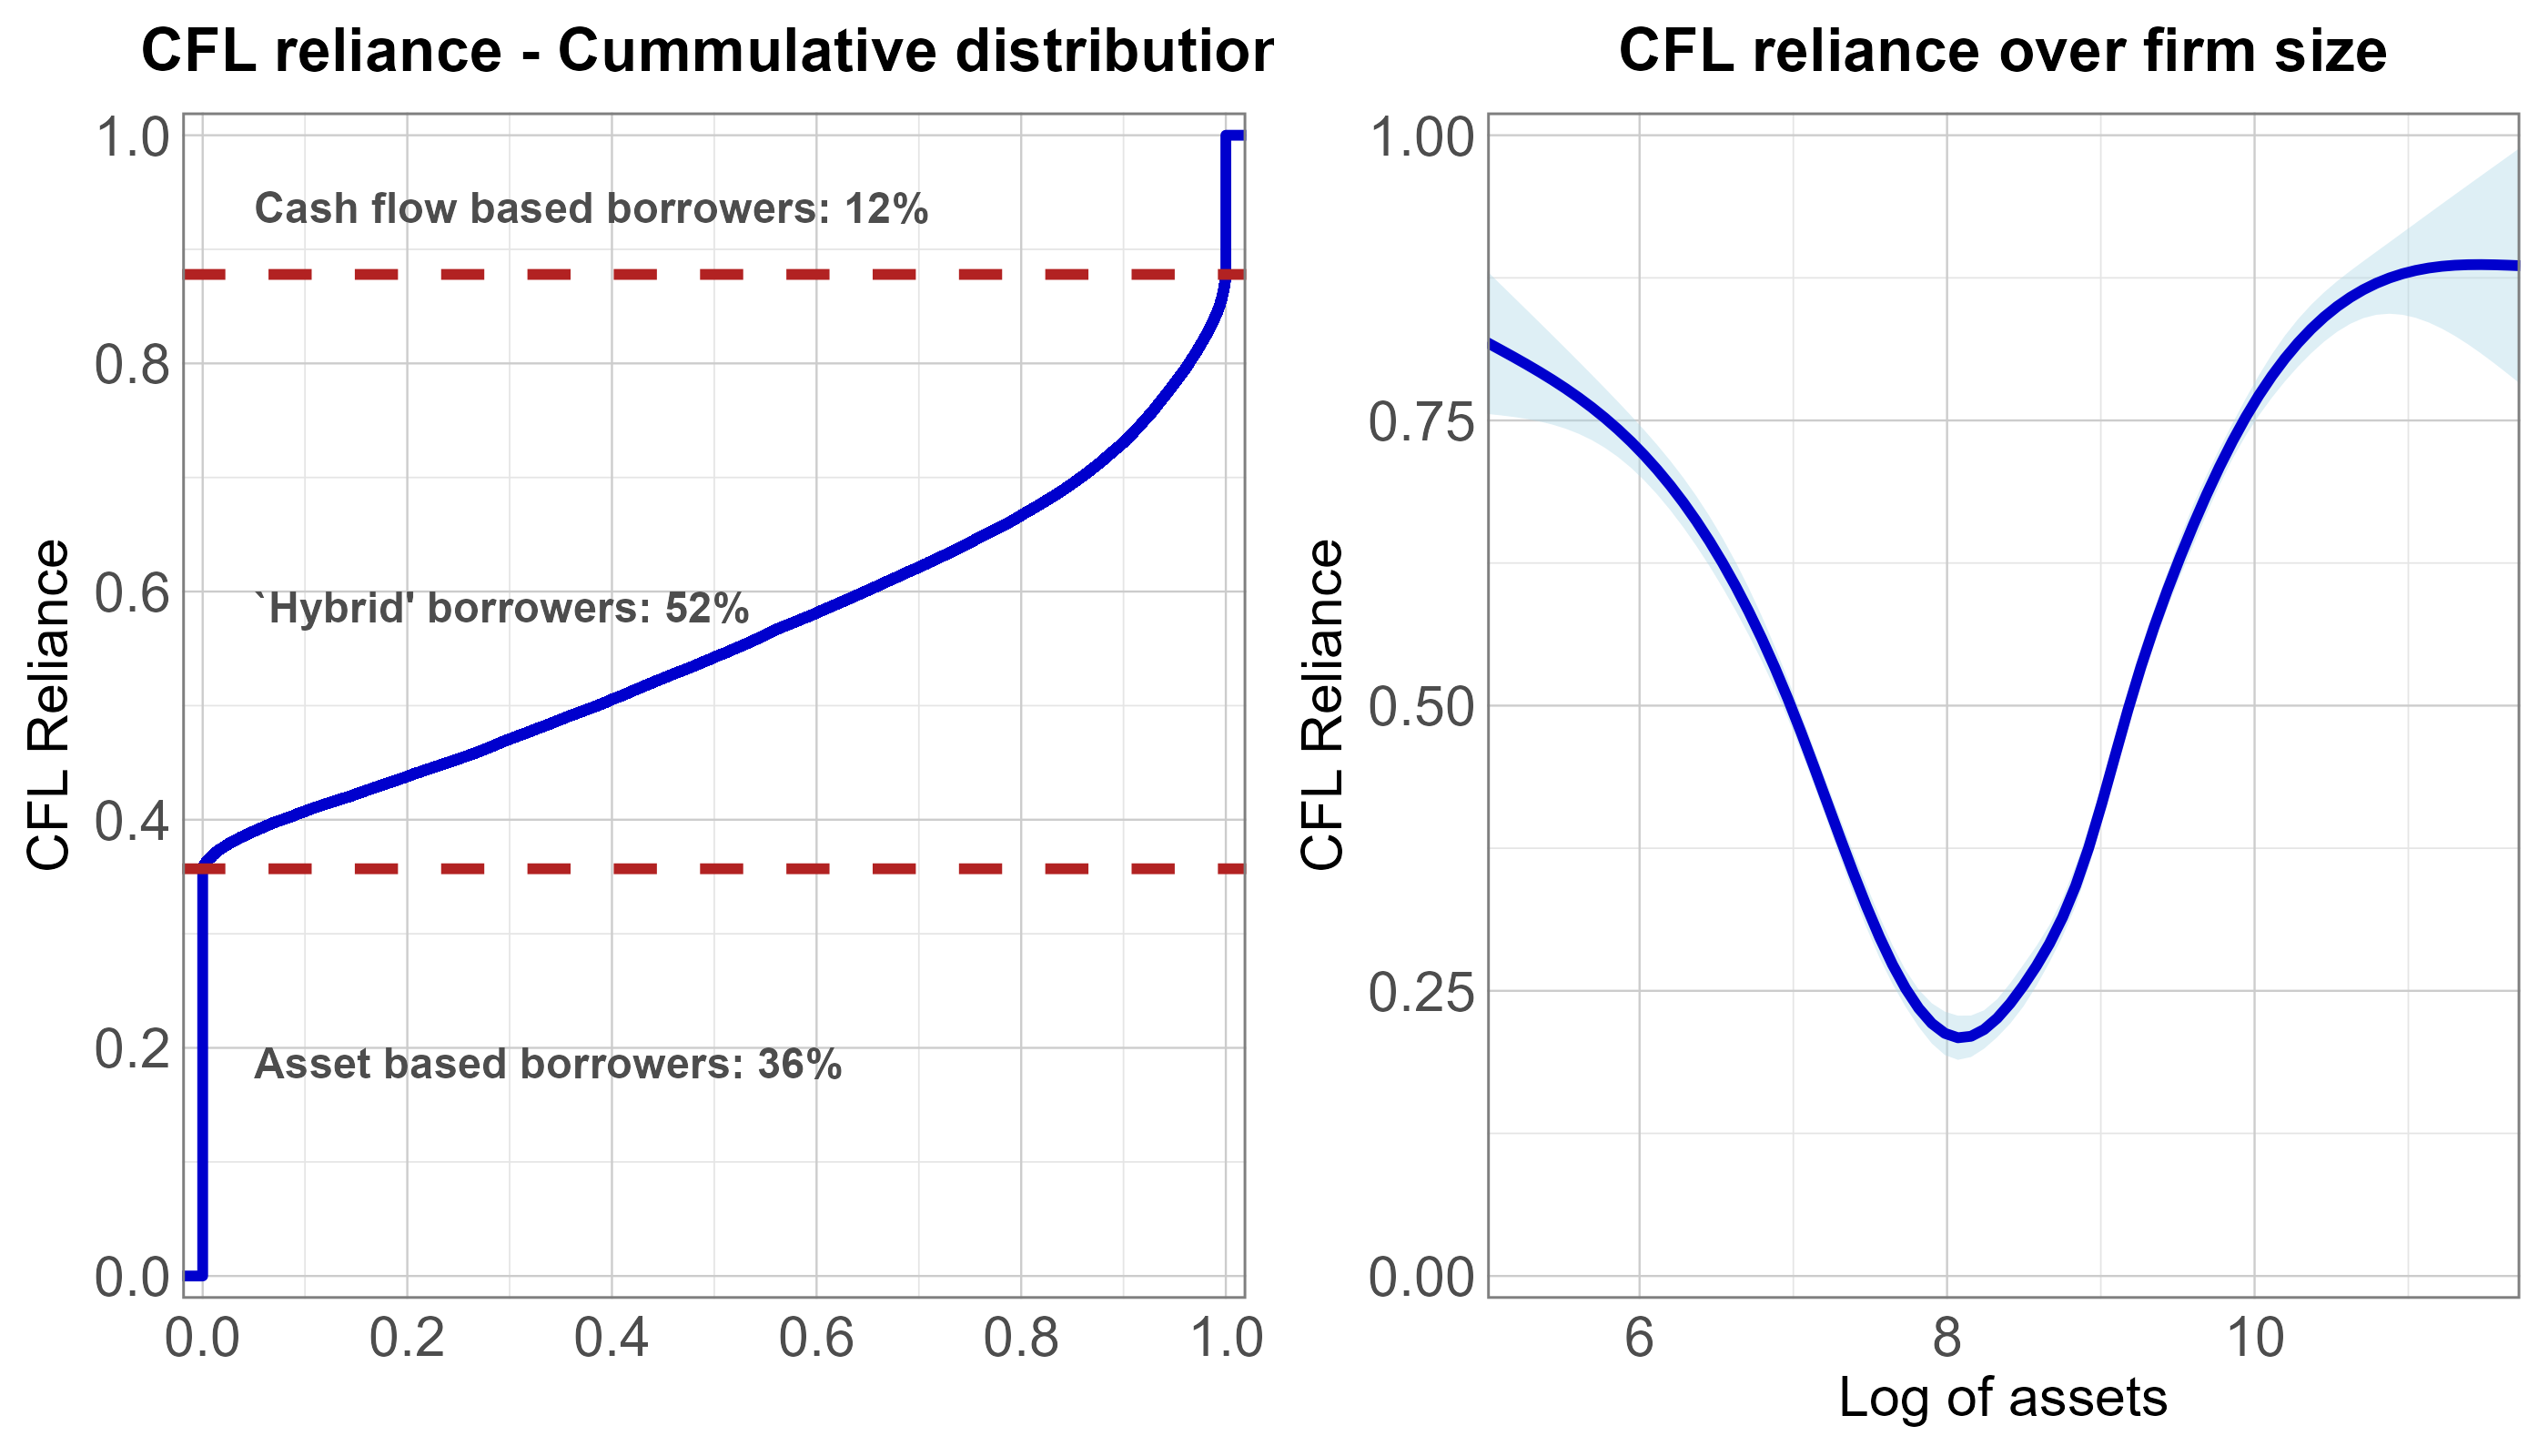
\includegraphics[width=1\textwidth]{smoothcfd.png}
     \begin{justify}
     \small Panel A. displays the cumulative distribution of CFL reliance. The horizontal dashed lines indicate the share of firms in each group of borrowers. Panel B. shows a moving average of CFL reliance across firm sizes, which is measured by the logarithm of assets. The red dots represent individual firms. 
    \end{justify}
\end{figure}

\noindent Panel A of figure \ref{chart:CFLcdf} provides additional details on the distribution of CFL reliance across firms. It shows that CFL reliance is particularly high for the largest and the smallest firms in the sample. In particular, plotting CFL reliance against firms size (measured by the logarithm of assets) yields a U-shape. This result is unique to indicators of firms size and remains robust over time and across sectors. Moreover, Orbis evidence suggest that it also holds for a wider set of countries, albeit not all - see figure \ref{chart:orb2} of the appendix. 

\subsection{Multivariate analyses \label{sec: multivariate analysis}}

In the previous section, I highlighted asset size as an important determinant CFL reliance. Prior studies have suggested various factors other than size that may influence the propensity to borrow against future cash flows. In this section, I explore the determinants of CF-based lending and test the robustness of previous findings. \vspace{3mm} \\
Asset-specificity and capital-intensity are also frequently highlighted as important determinants of cash flow-based borrowing, since firms that predominantly rely on intangible or illiquid assets may find it hard to pledge collateral (Lian and Ma, 2021). Another important determinant is the `institutional setting' comprising aspects such as the legal environment, court enforceability, reporting obligations and bankruptcy processes. Cross-country comparisons offer the most straightforward approach to study these factors. I study these considerations in more detail in section \ref{sec:A4} of the appendix.
 \vspace{3mm} \\
Table \ref{tab:regres} presents three regression results. Given that most potential determinants have incomplete or missing data points, there is a trade-off between adding explanatory variables and preserving the sample size. First, I discuss the results of a pooled OLS estimation with a wide set of regressors - this limits the studied sample size to 20\% of the original sample but allows us to study most potential determinants. The remaining regressions include fewer variables to preserve sample size as much as possible. The second column of table \ref{tab:regres}, studies within firm variation via fixed-effects regression. In the third regression, observations correspond to averages of individual firm characteristics over time. This regression is designed to explore on across-firm variation of CFL reliance. \vspace{3mm} \\
As argued by the previous section, firm size (measured by assets) is one the most important predictor of CFL reliance. To assess the robustness of the U-shaped pattern illustrated in figure \ref{chart:CFLcdf}, I include the square of the logarithm of assets in the regression. The coefficient for this variable is consistently positive and statistically significant in each regression, indicating the persistence of the U-shaped relationship. In isolation, log of revenue and employees display a similar pattern - see figure \ref{chart:CFL} in the appendix. However, once assets are accounted for, these variables become insignificant in most cases. This suggest that when borrowing strategy is concerned, the value assets is the best measure of firms size. \vspace{3mm} \\
Leverage also has strong (positive) effect on CFL reliance, which remains robust across different specifications. This implies the existence of a pecking order between asset-based and cash flow-based borrowing. Firms with relatively little debt compared to their size can cheaply access asset-based debt. In this case, there are no strong incentives to bear the additional fixed costs related to cash flow-based borrowing. However, as a firm accumulates more debt, lenders become reluctant to extend credit solely based on the prospect of seizing collateral in the event of default. At this point, cash flow-based borrowing becomes increasingly appealing to the company. \vspace{3mm} \\
I define asset pledgeability as the share of collateralizeable assets to total assets (precise Compustat definitions are detailed in section \ref{sec:A3} of the appendix). I find that higher asset pledgeability is associated with lower CFL reliance. Along with firm size and leverage, this indicator remains an important predictor of CFL reliance across all specifications. This is consistent with the hypothesis that companies holding intangible or less liquid assets are inclined to favor cash flow-based borrowing due to their inability to provide adequate collateral.  \vspace{3mm} \\
All else fixed, firm age is also positively associated with CFL reliance. One way to interpret this result is that lenders become less reluctant to lend against future cash flows when a firm has an established business model and reliable credit history. Alternatively, it could be associated to a pre-selection of firms: the type of firms that survive long, tend borrow against future cash flows more intensively. The sign of the age coefficient becomes negative when within-firm variation is considered. This indicates that the latter explanation is more likely. In summary, age by itself can play a significant role in determining cash flow-based lending (CFL) reliance.\footnote{Reproducing this observation in a structural model, would warrant a setup where lenders learn about firm characteristics over time via Bayesian updating. In this setup, accumulating information about the firm could lead to more lenient credit conditions in itself. To keep the model parsimonious, I choose not to incorporate this mechanism into the structural model.}
\vspace{3mm} \\
Indicators of profitability are either insignificant or have a negative effect on CFL reliance.  One possible explanation to this is the prevalence of CFL for large companies that do not realize large cash flow relative to their size. Moreover, as figure \ref{chart:CFL} in the appendix indicates, certain companies that experience significant losses frequently maintain cash flow-based contracts. In any event, this evidence does not support the view lenders simply extrapolate current earnings to estimate future expected cash flows. \vspace{3mm} \\
Instead, as I discuss in section \ref{sec:loan rates}, lenders must consider all discounted future cash flows. Hence, the perceived potential of the company matters more than its current profitability. Credit ratings can be interpreted as a proxy for this perception. Consistent with this view, results suggest that, firms with better credit rating (more favourable outsider perception) hold more CF-based debt. Another piece of evidence that points in this direction is that productivity, which measures the added value of the firm relative to its size, also consistently displays a positive and significant association with CFL reliance.  \vspace{3mm} \\
Finally, the significant and robust difference between US and Canadian firms' CFL reliance can be interpreted as evidence that institutional factors, such as bankruptcy codes, legal environment and reporting standards have a considerable impact on lending choices - I study further cross country comparisons in section \ref{sec:A4} of the appendix.

\begin{table}[H]
\centering
\label{tab:your_table_label}
\resizebox{\textwidth}{!}{%
\begin{tabular}{lcccccccc}
\toprule
& \multicolumn{3}{c}{POLS} & \multicolumn{3}{c}{FE regression} & \multicolumn{2}{c}{Firm level regression} \\
\cmidrule(lr){2-4} \cmidrule(lr){5-7} \cmidrule(lr){8-9}
LHS: CFL share & Value & SE & & Value & SE & & Value & SE \\
\midrule
Leverage & 0.176*** & (0.00662) & & 0.206*** & (0.0150) & & 0.244*** & (0.0155) \\
Pledgeability & -0.161*** & (0.0101) & & -0.174*** & (0.0297) & & -0.129*** & (0.0225) \\
Liquidity & 0.157*** & (0.0174) & & 0.0129 & (0.0256) & & -0.139*** & (0.0297) \\
Age & 0.00038*** & (4.96e-05) & &  -0.011*** & (0.0014)  & & 0.00057*** & (0.000126) \\
Log of employees & -0.0118*** & (0.00229) & & 0.00753 & (0.00753) & & -0.00238 & (0.00470) \\
Log of revenue & -0.000854 & (0.00293) & & 0.00326 & (0.00391) & & 0.00184 & (0.00453) \\
Log of assets & -1.059*** & (0.0289) & & -0.550*** & (0.0987) & & -1.321*** & (0.0647) \\
Log of assets squared & 0.0701*** & (0.00168) & & 0.0353*** & (0.00588) & & 0.0835*** & (0.00397)\\
Profit variance & & & & & & & -5.86e-08 & (9.80e-08) \\
Profitability & -0.44*** & (0.035) & & 0.035 & (0.033) & & -0.225*** & (0.059) \\
Productivity & 0.511*** & (0.0757) & & & & & 0.562*** & (0.200) \vspace{3mm} \\
 \multicolumn{9}{l}{\textbf{Industries} - baseline: Agriculture and Fishing} \\
Construction  & -0.0836*** & (0.0266) & & & & & 0.0946 & (0.0642) \\
Manufacturing & -0.0182 & (0.0236) & & & & & 0.0477 & (0.0541) \\
Mining & 0.0611** & (0.0241) & & & & & 0.155*** & (0.0554) \\
Retail trade & -0.129*** & (0.0246) & & & & & -0.0299 & (0.0561) \\
Services  & -0.124*** & (0.0239) & & & & & -0.00629 & (0.0548) \\
Public Util., Transport & -0.0935*** & (0.0244) & & & & & 0.0318 & (0.0567) \\
Wholesale Trade & -0.0628** & (0.0249) & & & & & 0.0150 & (0.0579) \vspace{2mm} \\
\multicolumn{9}{l}{\textbf{Countries}  - baseline: Canada} \\
United States & 0.0227*** & (0.00561) & & & & & 0.0397*** & (0.0115) \vspace{2mm} \\
 \multicolumn{9}{l}{\textbf{Credit ratings}  - baseline: A} \\
A+ & 0.0539*** & (0.0149) & & & & & & \\
A- & -0.0606*** & (0.0143) & & & & & & \\
B+ & -0.174*** & (0.0118) & & & & & & \\
B & -0.109*** & (0.0119) & & & & & & \\
B- & -0.205*** & (0.0117) & & & & & & \\
C & -0.203*** & (0.0119) & & & & & & \\
D & -0.101*** & (0.0146) & & & & & &  \vspace{2mm} \\
Constant & 4.468*** & (0.128) & & 3.027*** & (0.428) & & 5.393*** & (0.275) \\
\hline
Observations & 38,416 & & & 118,796 & & & 5,813 & \\
R-squared & 0.261 & & & 0.041 & & & 0.295 & \\
Number of companies & & & & 5,970 & & & & \\
\bottomrule
\multicolumn{9}{c}{*** p$<$0.01, ** p$<$0.05, * p$<$0.1} \\
\end{tabular}%
}
\caption{\small Explaining CFL reliance in 3 regressions}
\label{tab:regres}
\end{table}
\restoregeometry % Restore the default page layout

\noindent Taking stock of the empirical evidence, I highlight following results:
\begin{enumerate}[i]
    \item the majority of firms have asset-based as well as CF-based debt, implying that they typically encounter both types of financial frictions;
    \item the distribution of CFL-reliance is consistent with high fixed costs of lending against future cash flows;
    \item firm size, as measured by total assets of the company leverage and asset pledgeability are the main determinants of CFL reliance.
    \item When plotted against firms size, CFL reliance is U-shaped. This relationship persists in multivariate analyses.
\end{enumerate}

\section{Qualitative analysis of bankruptcy practices \label{sec: qualitative analysis}}
\subsection{Default resolution frameworks \label{sec: default resolutions}}
When debt is secured against collateral, the lender expects to retrieve in-default payments by liquidating borrowers’ physical assets. The absence of such securities in case of cash flow-based contracts reflects creditors’ expectation that financial distress will be resolved through the reorganization of the borrower. Hence, asset-based debt contracts are consistent with liquidation, whereas cash flow-based contracts can be associated with the expected reorganization of the borrower.  \vspace{3mm} \\
However, the terms of debt contracts must be established ex-ante, whereas decisions concerning default resolution are made ex-post, only if financial difficulties arise. To better understand the determinants of creditors' expected, in-default payoffs under different debt contracts, it is worth discussing bankruptcy practices in more detail. In the following, I highlight some key characteristics of the US bankruptcy codes that will later inform the structural model. Appendix \ref{sec:A1} offers a more complete discussion of US bankruptcy procedures and also draws comparisons with the EU bankruptcy codes. \vspace{3mm} \\
\textit{a) The decision to reorganize or liquidate initially lies with the debtor, but lenders may enforce the conversion of the case under certain conditions.} Bankruptcy codes typically expect the debtor to first file for liquidation or reorganization - hence, the initial decision is in the hand of the debtor. Creditors may apply for the conversion of the default resolution, but this is approved only under special circumstances. Overall, the influence of a single lender over the default resolution is limited. Hence, unless the creditor deems that the probability of liquidation is zero, the terms of the debt contract must reflect the liquidation value of the borrower as well.\footnote{When the debt is secured against `substantially all assets', the lender becomes the owner of the entire corporate entity and it can make the liquidation decision himself. However, even in this case, the lender may find it more profitable to liquidate the company under certain conditions.}  \vspace{3mm} \\
\textit{b) Reorganizations must comply with the `best-interest-of-creditors' test.} This rule states that no dissenting creditor should be worse off under the proposed reorganization plan than it would be under the liquidation of the debtor. I refer to this principle as a basis to exclude scenarios in the structural model where asset-based borrowers undergo reorganization. In such cases, lenders can consistently expect to recover at least the liquidation value of the firm, making it unnecessary to consider this possibility when establishing conditions for asset-based lending. \vspace{3mm} \\
\textit{c) Special provisions to facilitate reorganization of SMEs}. Bankruptcy codes often attempt to alleviate the reorganization costs for small enterprises.\footnote{The EU directive allows member states to introduce special provisions to speed up and simplify the reorganization process for SMEs. The US bankruptcy code allow SMEs to file for a small business case (11 U.S.C. § 101(51C)) or under subchapter V of the Small Business Reorganization Act (SBRA), both of which are intended to streamline the reorganization process and reduce costs.} This is based on the recognition that these costs are often prohibitive for small enterprises. Despite the special provisions in place, SMEs are still far more likely to choose liquidation. I interpret this as evidence for the high fixed costs of the reorganization process. Continuing

\subsection{The fixed costs of lending against cash flows \label{sec:fixed costs}}
In the previous section, I emphasized that the empirical evidence points to substantial fixed costs of lending against future cash flows. This section identifies two possible sources of fixed costs: the costs of reorganization which materialize only under financial distress and monitoring costs that creditors must pay on an ongoing basis in order to maintain a realistic on the debtors' going-concern value. \vspace{3mm} \\
The reorganization process involves a lengthy negotiation between debtors, creditors, and courts, which imposes significant costs on the involved parties. When in-default payments are expected to be enforced via reorganization, the lender must take into account the legal, personnel and time expenses of this process. The costs of reorganization may fall on the debtor and the creditor as well. I summarize all fixed costs that materialize under the reorganization process with the parameter $\zeta_1$. \vspace{3mm} \\
Maintaining a cash flow-based debt contract may impose significant costs on the lender even in the normal course of business. Asset-based contracts only require occasional evaluations and audits of the borrower's assets. In contrast, cash flow-based contracts require that the lender carries out its `due diligence' on an ongoing basis. The apparatus to maintain this monitoring activity may impose significant expenses for the lender.\footnote{This type of cost shares some similarities with the costly state verification first proposed by Towsend (1979). Although this concept had significant influence in the macro-finance literature, it is typically not mentioned in relation to cash flow-based contracts.} I summarize costs of CF-based lending, that materialize regardless of financial distress, by $\zeta_2$. More generally, this could be thought of as all additional expenses lenders face on a regular basis, when they deviate from standardized asset-based contracts. In the structural model, these fixed costs represent significant limitation in access to cash flow-based contracts. 

\section{Model outline \label{sec:model}}
\subsection{Firms and production \label{sec:production}}

A mass of heterogeneous is firms producing a homogeneous consumption good, using labour, $n$ and capital, $k$. Firms are competitive, and face a decreasing returns to scale production technology:
\begin{equation} \label{eq:prodf}
y = \varepsilon k^{\alpha}n^{\nu}, \ \ \ \ \alpha,\nu \in (0,1),  \ \nu + \alpha \in (0,1)
\end{equation}  
where $\varepsilon$ is the idiosyncratic productivity state. In the interest of keeping the notation simple, I omit firm subscripts. \vspace{3mm} \\
Firms own capital and investments are financed partly by financial wealth and partly by borrowing from a competitive lender. A firm can be described by the predetermined capital stock $k \in \mathbf{K} \subset \mathbf{R^{+}}$, debt\footnote{Firms may also decide to save in which case their debt towards the intermediary is negative.} $b \in \mathbf{B} \subset \mathbf{R}$ and current productivity $\varepsilon \subset \mathbf{R^+}$. Idiosyncratic productivity is a Markov chain on a finite set $\varepsilon \in \mathbf{E} \equiv \{ \varepsilon_1,...,\varepsilon_{N_{\varepsilon}} \}$ such that $ g_{ij} \equiv \Pr(\varepsilon'= \varepsilon_j|\varepsilon = \varepsilon) \geq 0$ and $\sum_{j=1}^{N_{\varepsilon}} g_{ij} = 1$ for each $i$. Moreover, it is stochastically monotone such that for any fixed $x$, $\Pr(\varepsilon' \leq x | \varepsilon = \varepsilon_i)$ is decreasing in $\varepsilon_i$. \vspace{3mm} \\
Production occurs before the realization of exit and entry decisions take effect, and optimal labor demand is independent of current debt. Therefore, every firm with the state vector at the beginning of the period $(k,\varepsilon)$ faces the same static optimization of labour: 
$$ \pi(k,\varepsilon) = \max_{n} \ \  \varepsilon k^{\alpha}n^{\nu} - wn - c$$
where $c$ is a fixed cost of participating in production, $w$ is equilibrium wage and the price of the consumption good is flexible and normalized to $1$. Optimization yields the policy function for labour demand, $n(\varepsilon,k)$ and optimal production $y(\varepsilon,k)$: 
\begin{equation} \label{eq:opt_emp_prod}
n(k,\varepsilon) = \left( \dfrac{ \nu \varepsilon k^\alpha}{w} \right)^{\frac{1}{1-\nu}} \hspace{15mm}
y(k,\varepsilon) = \varepsilon k^{\alpha} \left( \dfrac{\nu \varepsilon k^\alpha}{w} \right)^{\frac{\nu}{1-\nu}}
\end{equation}  
Firm profit function can be reformulated as: 
\begin{equation} \label{eq:profit}
\pi(k,\varepsilon) = y(k,\varepsilon) - wn(k,\varepsilon) - c = (1-\nu) y(k,\varepsilon) - c
\end{equation} 
Active firms own capital and make idiosyncratic investment decisions. Capital accumulation follows: 
\begin{equation} \label{eq:capital}
k' = (1-\delta)k + i
\end{equation} 
where $\delta$ is the depreciation rate and $i$ is investment. Capital adjustment is not subject to microeconomic frictions. Moreover, the lending schedule faced by individual firms depends only on future values of capital and debt, which firms may choose independently from current stocks. Hence, firms' financial position at any given period can be summarized by a cash on hand variable, $x \in \mathbf{X}$: 
\begin{equation} \label{eq:cash on hand}
    x = \pi(k,\varepsilon) + (1-\delta)k - b 
\end{equation}
The cash on hand and current productivity, $(x, \varepsilon)$ describe firms' current state. Hence, it is possible summarize the distribution of firms using the probability measure $\mu$ defined on the Borel algebra $A$, generated by the open subsets of the product spaces $ \mathbf{A} = \mathbf{X} \times \mathbf{E} $.  This reformulation reduces the computational burden the model. 


\subsection{Default and firm values \label{defaults}} 
Production takes places at the beginning of the period. Firms set their labour demand given $(k,\varepsilon)$, profits are realized and capital depreciates. After production, firms may experience an exogenous financial distress shock that is distributed uniformly across firms with probability $P_D$.\footnote{Introducing heterogeneity in default probabilities is not necessary to realize heterogeneity in debt contracts.} Under financial distress, the firm declares bankruptcy, which is associated with zero value regardless of the prior state or the eventual default resolution. Therefore, the continuation value is discounted with the probability of default: 
\begin{equation} \label{eq:V_0}
V_0(x,\varepsilon) = (1-P_\chi) V_1(x,\varepsilon)
\end{equation}
I define the indicator function $\chi_0$ which takes the value $1$ if the firm is reached by the insolvency shock and 0 otherwise. \vspace{3mm} \\
If the financial distress does not occur, the firm may decide to exit voluntarily. In this case, it retains the value of the depreciated capital stock net of debt service - i.e. the cash on hand. Let $V_1(x,\varepsilon)$ be the value of the firm before the voluntary exit decision is made. The firm chooses to exit if the current cash on hand exceeds the value associated with further production:
\begin{equation} \label{eq:V_1}
V_1(x,\varepsilon) = \max \Big\{ V_2(x,\varepsilon), \ x \Big\}
\end{equation} 
where $V_2(x,\varepsilon)$ is the value associated with further production. I define the indicator function $\chi_1$ which takes the value $1$ if the firms exits voluntarily and 0 otherwise. \vspace{3mm} \\
Firms that survive to the next period have access to external finance in the form of one-period debt contracts. For every unit of debt to be repaid in the next period, they receive $q$ units of output that may be allocated towards investment or distributed as dividends. It is possible to borrow against physical assets or future cash flows. These debt contracts are distinguished by different in-default payoffs. In particular, asset-based contracts are yield better pay-offs under liquidation and CF-based contacts extract more value under reorganization - I discuss this in detail in the following section. In every other respect, the two kind of debt are perfect substitutes, such that total debt is: $b = b^C+b^A$. Analogously to the empirical analysis, I define CFL reliance as: 
\begin{equation}
    \tau = b^C/(b^C+b^A).
\end{equation}
In summary, continuing firms choose future capital stock, $k'$, total future debt, $b'$ and debt financing strategy $\tau'$ to maximize the discounted sum of dividends, $d$ 
\begin{equation} \label{eq:dividends}
d = x - k' +  q(k',b',\varepsilon, \tau')b'
\end{equation} 
The value of further production is associated with the Bellman equation: 
\begin{equation} 
    V_2(x,\varepsilon) = \max_{k',b', \tau'} \left(x - k' +  q(k',b',\varepsilon, \tau')b' + \beta \E_{\varepsilon'|\varepsilon} V_0(x',\varepsilon') \right)
\end{equation}
subject to: 
\begin{equation}
x' = \pi(k',\varepsilon')+(1-\delta)k'-b' \hspace{5mm} \text{and} \hspace{5mm} d \geq 0
\end{equation}

\subsection{Financial intermediation}
\subsubsection{Default resolution}
Default resolution entails negotiations between the borrower and multiple creditors (with potentially conflicting interests), with the supervision of courts. Moreover, the negotiating parties' bargaining power may depend on the specific terms outlined in the contract. Hence, I do not attempt a comprehensive description of bankruptcy proceedings under different debt contracts. Instead, I focus on providing an accurate account of lenders' expected costs and pay-offs when debt is backed by assets or future cash flows. A substantial part of this analysis revolves around these costs and payoffs as they play a crucial role in shaping the debt schedule offered by lenders. \vspace{3mm} \\
Bankruptcy may be resolved either through liquidation or reorganization. Liquidation entails that the firm exits and the its undepreciated capital stock is liquidated at total cost of $(1-\phi_A)k$. The remainder is distributed between the household and the lender. Under reorganization, the household (who owns firms) pays the lender in order to keep to firm on the market. The total cost of reorganization is $ (1-\phi_C) V + \zeta$, where $\phi_C$ is the variable cost of reorganization and $\zeta$ denotes fixed costs discussed in section ... . \vspace{3mm} \\
Reorganization is efficient, such that it maximizes the remaining value (collateral or continuation) of the firm. Let $\chi_D = 1$ if the firm is liquidated under financial distress. Then,
\begin{equation} \label{eq:liquidation decision}
    \chi_D =  \mathds{1}(\phi_A (1-\delta) k  \  \geq \ \phi_C V_2(x,\varepsilon)- \zeta)  
\end{equation}

\subsubsection{The lender's problem}
The opportunity cost of lending to corporations is determined by the risk-free bond yields $q_0$. Since corporate lending is inherently risky, the competitive lender must charge a premium to break even. To set $q(k',b',\varepsilon, \tau')$ the lender considers the expected payoff under 3 distinct scenarios: \textit{a)} orderly repayment; \textit{b)} the firms is liquidated under financial distress; \textit{c)} the firms is reorganized under financial distress. From equation \ref{eq:liquidation decision}, it is possible to determine the probability that the firm will be liquidated under financial distress as follows: 
\begin{equation} \label{eq:liquidation probability}
    \gamma(k',b',\varepsilon) = \E_{\varepsilon'|\varepsilon}[\mathds{1}(\phi_A (1-\delta) k'  \  \geq \ \phi_C V_2(x',\varepsilon')- \zeta)]  
\end{equation}
It follows from the zero-profit condition that the debt schedule offered to firms is, \textbf{here you need a min function but only for one!} It should be $P_D(min(b, \gamma \Pi_{liq} + (1-\gamma)\Pi_{reorg}))$. \textbf{Finally, you should maybe rewrite the following with the CD model.}
\begin{equation} \label{eq:q}
    \begin{split}
        & q(k',b', \varepsilon, \tau')b' =  \beta \left[ (1-P_D)b' + \right. \\
        & \quad P_D \gamma(k',b',\varepsilon) \Pi_{liq}(k',b', \tau') +  \\
        & \quad \left. P_D (1-\gamma(k',b',\varepsilon)) \E_{\varepsilon'|\varepsilon} \Pi_{reorg}(k',b', \varepsilon', \tau') \right] 
    \end{split}
 \end{equation}
where $\Pi_{liq}$ and $\Pi_{reorg}$ denote the expected payoff under liquidation and reorganization. The next section discusses these in-default payoffs of the lender. 

\subsubsection{In-default payoffs}
Default resolution involves reallocating the remaining value (either collateral or continuation) of the firm in bankruptcy between lenders and the household. The debt financing strategy adopted prior to bankruptcy influences this redistribution.  \vspace{3mm} \\
When debt is secured against physical assets, the lender can enforce in-default payments by seizing and liquidating collateral. Thus, when the firm undergoes liquidation the lender can extract the full liquidation value $\phi_A (1-\delta) k$. Assessing the lender's payoff in the case of reorganization is not as straightforward, since asset-based contracts lack provisions that allow retrieving future cash flows. However, the lender is protected by the `best interest of creditor' test (see section ...), which states that creditors cannot be worse off under the reorganization plan than they would be in case of liquidation of the firm. Therefore, I assume that lender expect to be able to extract the same $\phi_A (1-\delta) k$ payment after asset-backed debt contracts when the firms is reorganized. \vspace{3mm} \\
In contrast, CF-based debt is not secured by collateral, hence the lender can expect to retrieve only a small fraction $\kappa$ of the original liquidation value when the lenders is liquidated. Therefore, lenders must expect in-default payments chiefly from the reorganization of the borrower. Moreover, cash flow-based debt contracts often contain provisions that allow lenders to directly recover a portion of the going-concern value of the borrower. Thus,  the lender can expect to retrieve some of the continuation value $\phi_C V(k,b,\varepsilon)$, when the borrower undergoes reorganization. Table \ref{tab:lender payoffs} summarizes lenders payoffs under each debt contract and default resolution: \\
\begin{table}[h!]
    \centering
    \begin{tabular}{l|cc}
        & Liquidation  & Reorganization \\  
       \midrule
      Asset based contract & $ \phi_A (1-\delta) k$  &  $ \phi_A (1-\delta) k$ \\
      CF based contract & $ \kappa \phi_A (1-\delta) k$ & $ \phi_C V(x,\varepsilon)$ \\ 
     \bottomrule
     \end{tabular}
    \caption{\small The lender's maximum potential payoffs under each default resolution-debt contract pair - gross of reorganization costs.} 
    \label{tab:lender payoffs}
\end{table}

\noindent With the information summarized in table \ref{tab:lender payoffs}, it is possible to outline the lender's expected payoffs when the lender undergoes liquidation or reorganization - $\Pi_{liq}$ and $\Pi_{reorg}$. Take liquidation first. The total liquidation value of the firm (i.e. the resale value of assets) is: $\phi_A (1-\delta) k'$. However, the lender can only retrieve this value for the  debt that is backed by collateral, which is $1-\tau$ share of the total debt. After the remaining $\tau$ share of the debt, the lender can only only seize $\kappa$ fraction of original liquidation value. In summary, the lender can expect the in-default payoff under liquidation of, \textbf{rewrite this without the min function.}
\begin{equation} \label{eq:P_liq} 
   \Pi_{liq}(k,b,\tau) = \min\{b, \ (1-\tau) \phi_A (1-\delta) k +\tau \kappa \phi_A  (1-\delta) k \}
\end{equation}
The minimum function indicates that the lender cannot recover more than the total value of the debt contract. Also note that the value retrieved under liquidation does not depend on the realization of idiosyncratic productivity. The value not claimed by the lender is redistributed to the household in the form of lump-sum transfer.\footnote{This amounts to: $ \max \{\phi_A (1-\delta) k - b, \hspace{1mm} \tau (\phi_A-\phi_C) k  \} $.} \vspace{3mm} \\
When the firms is reorganized, the household (the owner of the firm) pays the lender some fraction of the original firm value to keep the firm on the market. As discussed above, CF-backed debt contracts allow lenders to directly extract $\phi_C$ share of the continuation value. Moreover, the reorganization process incurs fixed costs, $\zeta$. When the lender expects in-default payments from reorganization, it must consider the that a portion of these costs may be incurred by her. In the following, I assume that lenders must pay these $\tau$ share of these fixed costs.\footnote{This is a relatively innocuous assumption. Lenders' expenses raise the costs of external finance premium of CF-based debt directly, whereas firms' costs raises the probability of resolving default via liquidation, which the raises costs of CF-based lending indirectly. Hence, the incidence of these costs has little effect on the external finance premium.} In accordance with the `best interest of creditors test', the lender expects to retrieve a payment that is equal to the liquidation value of the collateral after its asset-based debt. Taking stock, when the borrower undergoes reorganization, the lender receives \textbf{should add en extra min function}
\begin{equation}  \label{eq:P_reorg}
   \Pi_{reorg}(k,b,\varepsilon,\tau) = \min\Big{\{}b, \ (1-\tau) \phi_A (1-\delta) k +\tau \left( \phi_C V_2 (x, \varepsilon) - \zeta \right) \Big{\}}.
\end{equation}
The household pays the lender in a lump-sum transfer.\footnote{This amounts transfer to: $$ \max \{b - [(1- \phi_v) V_2 (x, \varepsilon) + \zeta)], (1-\tau)\phi_A(1-\delta)k + \tau V_2 (x, \varepsilon) + (1-\tau) [(1- \phi_v) V_2 (x, \varepsilon) + \zeta)]\}  $$} \vspace{3mm} \\
In practice, extracting the continuation value may differ depending on the debt contract that is in place. When debt is secured against the entire corporate entity or equity, the lender can directly obtain ownership in the firm. In his case, it may directly seize future cash flows (and it gains direct influence on the liquidation decision). When the debt is unsecured, the lender has fewer devices to collect future cash flows. Nevertheless, in the absence of collateral, lenders pay-offs will chiefly depend on the continuation of the defaulted firm.\footnote{Corbae and D'Erasmo (2021) consider a Nash bargaining game for debt renegotiation. The threat of liquidation forces firms with high continuation value to agree to more generous terms of repayment. This implies that in default payments depend positively on the continuation value.} Therefore, in line with previous literature, I classify unsecured debt contracts as CF-based. 
\subsubsection{Optimal debt financing strategy}
It follows from the assumption that firms associate zero value with bankruptcy that debt financing strategy (i.e. the choice of $\tau'$) only affects firm values through the current external finance premium. Moreover, since firm value is increasing in $q(k',b',\varepsilon, \tau')$, for any $(k',b',\varepsilon)$ the optimal debt financing strategy coincides with the $\tau'$ that maximizes the inverse gross interest rate. Substituting equation \ref{eq:P_liq} and \ref{eq:P_reorg} into \ref{eq:q} and using that in the stationary equilibrium $q_0 = \beta$, we can express the optimal CFL reliance as follows: \textbf{Rewrite with a single min}
\begin{equation} \label{eq:opt_tau}
    \begin{split}
        & \tau^*(k',b',\varepsilon) = \argmax_{\tau'} \ \  \frac{\beta}{b'} \Big{[} (1-P_D)b' \ +  \\
        & \quad  P_D \gamma(k',b',\varepsilon) \min\{b', \ (1-\tau') \phi_A (1-\delta) k' +\tau' \kappa \phi_A  (1-\delta) k' \} \ +  \\
        & \quad P_D (1-\gamma(k',b',\varepsilon))  \min\big{\{}b', \ (1-\tau') \phi_A (1-\delta) k' +\tau' \left( \phi_C \E_{\varepsilon'|\varepsilon}V_2 (x', \varepsilon') - \zeta \right) \big{\}} \Big{]} 
    \end{split}
 \end{equation}
Therefore, firms dynamic problem can be reformulated as, 
\begin{equation} \label{eq:V_2}
    V_2(x,\varepsilon) = \max_{k',b'} \left(x - k' +  q(k',b',\varepsilon, \tau')b' + \beta \E_{\varepsilon'|\varepsilon} V_0(x',\varepsilon') \right)
    \end{equation}
    subject to: 
    \begin{equation} \label{eq:cont_1}
    x' = \pi(k',\varepsilon')+(1-\delta)k'-b'; \hspace{10mm} d \geq 0;  \hspace{10mm} \tau' = \tau^*(k',b',\varepsilon)
    \end{equation}
    
\subsection{Firm dynamics}
In the previous sections, I defined the following indicator functions: $\chi_0 = 1$ if the insolvency shock materializes, $\chi_1 = 1$ if the firm is voluntarily liquidated, $\chi^D = 1$ if it is liquidated under financial distress. The combinations of these indicator functions describe the possible resolutions the debt contract, summarizted by \ref{table:indic}. Taking stock of liquidations, a firm may be liquidated voluntarily: $(1-\chi_0)\chi_1 = 1$ or under financial distress: $\chi_0\chi^D = 1$. These cases represent firms exits in the model. \vspace{3mm}\\
At every period, exits are balanced by a mass of entrants. These are endowed with a starting cash on hand and productivity drawn from the distribution $\Phi(x,\varepsilon)$. To reflect the fact that startup companies are typically asset-poor, this distribution is defined to yield low cash on hand on values relative to incumbent firms. The entry decision is described by equation \ref{eq:V_1}: potential entrants enter only if the continuation value is higher than their startup cost.\footnote{Entrants only start producing in the next period, hence their profits in the cash on hand variable is zero.} I define $\chi_e$ be equal to one if the potential entrant decides to enter and zero otherwise. 

\begin{table}[h!]
    \centering
    \begin{tabular}{|c|c|c|c|} 
    \hline
    Case &$\chi_0 $ - insolvency & $\chi_1, \ \chi_1^D$ - liquidation &  Outcome  \\ \hline
    1. & $\chi_0 = 0 $ &  $\chi_1 = 0$  & Repays debt, Continues \\
    2. & $\chi_0 = 0$ &  $\chi_1 = 1 $  & Repays debt, exits   \\
    3. & $\chi_0 = 1$ &  $\chi_1^D = 0$  & Insolvent, Reorganized  \\
    4. & $\chi_0 = 1$ &  $\chi_1^D = 1$ & Insolvent, Liquidated \\ 
    \hline
    \end{tabular}
    \caption{Possible debt contract resolutions in the model}
    \label{table:indic}
\end{table}
    
 \noindent Production takes place at the beginning of the period, therefore the measure, $\mu$ describes to the mass of active firms at any given time. Let $\overline{\mu}$ denote the measure of firms that are present at the end of the period. At each period, this evolves according to $ \overline{\mu} = (1-(1-\chi_0)\chi_1-\chi_0\chi^D) \mu + M \chi_{e} \ d \Phi$. The evolution of firm distribution then satisfies:
\begin{equation} \label{eq_firmdim} 
    \mu'(A) = \int \mathbf{I}_{(x', \varepsilon') \in A} g(\varepsilon'|\varepsilon) \ d \  \overline{\mu} (x,\varepsilon)
\end{equation}
for all Borel sets $A \subset  \mathbf{X} \times \mathbf{E} $ and where $g(\varepsilon'|\varepsilon)$ is the transition probability matrix idiosyncratic productivity. I summarize firm dynamics of firm distribution at the beginning of the period by the mapping $ \mu' =\Gamma(\mu)$.

\subsection{Households}\label{sec:hh}
Households choose consumption, $C$ labour, $L$ and non-contingent bonds, $B$ to maximize expected discounted utility - these yield the gross interest rate $1/q_0$. Moreover, households own all firms, which implies that they realize revenues and expenses from the production sector. On the revenue side, households receive dividends and the net wealth of firms that are liquidated voluntarily. On the expense side, households must endow entrants with starting capital, and re-buy firms that are reorganized by the financial intermediary. Moreover households receive lump-sum transfers $T$, that summarize costs and payoffs related to financial intermediation - these are summarized in section ... . These expenses and gains are pooled among households, hence the maximization problem:
\begin{equation} \label{eq:U_max}
V(B, \mu) = \max_{C,L,B'} U(C, 1-L) + \beta V(B', \mu')
\end{equation}  
subject to: 
\begin{multline} \label{eq:const_hh}
C + B + M \int  \chi_e (k-b) \ d \Phi(x,\varepsilon)  \leq wL + q_0 B' + T + \\  \int (1 - \chi_0) \chi_1 \ x \ d \mu(x,\varepsilon) + \int (1-(1-\chi_0)\chi_1-\chi_0\chi^D) \left( x - k'(x,\varepsilon) + qb'(x,\varepsilon) \right) d \mu(x,\varepsilon)
\end{multline} 
and given the evolution firm distribution measure: $\mu' = \Gamma(\mu)$. Transfers collect leftover capital value after involuntary liquidations and payment to the intermediary after reorganized firms. In total this amounts to 
\begin{multline*} \label{eq:T}
    T = \int \chi_0\chi^D  \max \{\phi_A (1-\delta) k - b, \hspace{1mm} \tau (\phi_A-\phi_C) k  \}  + \\
    \int \chi_0(1-\chi^D) \max \big{\{}b - [(1- \phi_v) V_2 (x, \varepsilon) + \zeta)], \\ (1-\tau)\phi_A(1-\delta)k + \tau V_2 (x, \varepsilon) + (1-\tau) [(1- \phi_v) V_2 (x, \varepsilon) + \zeta)]\big{\}} 
\end{multline*} 
Let the $C(b,\mu)$, $N(b,\mu)$, $B(b,\mu)$ be the policy functions for consumption, labour and next bond holdings in the next period. 

\subsection{Stationary equilibrium}\label{sec:eq}
The stationary competitive equilibrium can be described by the set of functions
$$(\mu, w, V_0, V_1, V_2, \chi^0, \chi^1, \chi^D, \chi^e, l,q,k,b,d, V_h, C, N, B)$$
such that: 
\begin{enumerate}[(i)]
\item Firms solve value maximization: $V_0$, $V_1$ solves \ref{eq:V_0}, \ref{eq:V_1} respectively and $V_2$ solves \ref{eq:V_2} and \ref{eq:cont_1} and the associated policy functions are $l$, for exiting firms and $(l,k,b,d,q)$ for entering and continuing firms
\item Households solve utility maximization: $V_h$ solves \ref{eq:U_max}-\ref{eq:const_hh} and the associated policy functions are $( C, N, B)$
\item Labour market clears: 
$$ N = \int n  \ d \mu (x,\varepsilon)  $$
\item Financial market clears:
 $$ B = \int b \ d \mu (x,\varepsilon) $$
\item Goods market clear: 
$$ C + I = \int y \ d \mu (x,\varepsilon)$$
where aggregate investment is the sum of investment carried out by continuing firms and startups minus the capital freed up due to voluntary and involuntary liquidations:
\begin{multline*} 
    I = \int (1-(1-\chi_0)\chi_1-\chi_0\chi^D)\left[ k' -(1-\delta)k \right] d \mu (x,\varepsilon) - \\
    \int \chi_0\chi^D (1-\delta) \phi_A k \ d \mu (x,\varepsilon) \int (1-\chi_0)\chi_1(1-\delta) k \ d \mu (x,\varepsilon)  + M \int \chi_e k \ d \Phi(x,\varepsilon) 
\end{multline*}
\item The distribution measure of active firms is stationary, $\Gamma(\mu) = \mu$ and prices $(w,q)$ are constant over time.
\end{enumerate}

\section{Conclusion \label{Concl}}
I study the debt financing strategies of North American, traded non-financial corporations. Most firms hold multiple debt contracts, which often comprise a combination of asset-based and cash flow-based debt.  This implies credit market frictions are better described as a combination of asset-based and earnings-based constraints. In order to provide a precise description of the nature of these credit constraints, I explore the determinants of firms’ debt financing strategies along these lines. \vspace{3mm} \\
First, I study the extent to which North American, listed non-financial corporations rely on CF-based borrowing. The main determinants are size of assets, leverage and the share of collateralizable assets on the balance sheet. Moreover, the distribution of CFL reliance can be best explained by substantial fixed costs of lending against future cash flows. This confirmed by a qualitative analysis of bankruptcy procedures. In the case of CF-based lending, two sources of fixed costs stand out: the potential expenses of the reorganization process and expenses that relate to monitoring borrowers’ potential future cash flows on an ongoing basis. \vspace{3mm} \\
The second part consolidates these findings in a structural model, where firms are heterogeneous in productivity own capital and may borrow or save. This framework is complex enough to account for most major determinants influencing the reliance on cash flow-based lending. The purpose of this exercise is twofold. First, it explores the degree to which fixed costs account for the key patterns observed in firms' debt financing strategies. Second, it offers a precise description of credit frictions and their effects on the wider economy.

\setcounter{table}{0}
\setcounter{figure}{0}
\setcounter{section}{0}

\section{Appendix \label{sec:appendix}}
\subsection{Bankruptcy frameworks in the US and EU  \label{sec:A1}}

The US Bankruptcy Code is structured into chapters, each corresponding to a different type of relief for debtors in financial distress. In particular, chapter 7 deals with liquidations and chapter 11 regulates the reorganization process. The European Union does not have a single bankruptcy code, but it has been working towards harmonizing insolvency proceedings across member states, based on the understanding that divergent insolvency laws create barriers across member states. As a result, the Harmonisation Directive\footnote{Directive (EU) 2019/1023 of the European Parliament and of the Council of 20 June 2019 on preventive restructuring frameworks, on discharge of debt and disqualifications, and on measures to increase the efficiency of procedures concerning restructuring, insolvency and discharge of debt.}  was published in June 2019, and member states are required to adopt the necessary legislative changes by July 2021 to comply with it. Although it does not completely standardize bankruptcy procedures, the directive outlines several principles that mirror the main features of chapter 7 and 11 of the US bankruptcy code. It represents a valuable piece of evidence for this discussion, as it collects the set of principles that legislators aim to institute in bankruptcy proceedings. \vspace{3mm} \\
Under both frameworks, the debtor is expected to file for insolvency – although creditors may petition the court to initiate bankruptcy proceedings against the debtor, this is not the norm. Hence, the decision to pursue reorganization or liquidation initially lies with the debtor. If the debtor decides to draft a reorganization plan, creditors may form committees and have their claims heard by courts. The European Union has a more debtor-friendly approach, meaning that creditors have less influence over the outcome of the proceedings, whereas the US system places more weight on the interest of the creditors. However, it is often the case that a debtor has numerous creditors, which limits the influence of any individual creditor over the specifics of the bankruptcy proceedings. \vspace{3mm} \\
One exception to this rule, is that no dissenting creditor should be worse off under the proposed reorganization plan than it would be in case of liquidation. The EU Directive refers this as ‘best-interest-of-creditors’ test in OJ L 172/27, art. 49; whereas the US bankruptcy code establishes this principle in 11 U.S. Code § 1129.  If the reorganization plan fails this test, it may not receive the necessary court approval (the dissenting creditor is entitled to vote against it). In the context of the model, this becomes relevant when an asset-based borrower decides to file for reorganization. The lender cannot receive a lower payoff than it expects to see from the liquidation of collateral (although it might have to pay some legal fees). Thus, from the point of view of the asset-based lender it does not matter if the borrower wishes to continue operating after the bankruptcy have been resolved. As discussed in section \ref{sec: qualitative analysis}, I abstract from these cases altogether.  \vspace{3mm} \\
Creditors have even less influence when a borrower seeks to resolve financial distress through liquidation of its assets - as it would be unrealistic to expect the firm to continue operating against the best judgement of its management. An important exception from this rule is when the debt is secured against the entire corporate entity. In this case, the creditor can take over the firm in case of default and may decide freely between reorganization and liquidation. Yet, cash flow-based lenders must take into account that in case of a default, they may only retrieve the liquidation value of the collateral.  This outcome could arise from mutual creditor-debtor agreement. Alternatively, it may reflect debtors' choice, possibly conflicting with the creditor's best interests. Hence, the risk premium on these loans will reflect the `Chapter 7 outcome’ too unless the lender deems that the probability of reorganization is negligible. 

\subsection{Data appendix \label{sec:A3}}
\subsubsection{Compustat and Capital IQ}
Compustat is a comprehensive, financial database maintained by S\&P Global. It offers standardized firm-level information on publicly traded companies compiled from financial statements, regulatory filings and other financial reports. I use the quarterly tables in Compustat North America which chiefly contains US and Canadian corporations. Moreover, I exclude financial corporations (SIC code 6000 to 6799) and utility providers (SIC code 4900-4999) from the sample. S\&P Capital IQ offers an extensive array of debt-level statistics. The two datasets can be connected via the unique firm a identifier (GVKEY), moreover Capital IQ covers most of the Compustat firms and yields consistent firm-level debt data after the aggregation of debt contracts. Although Capital IQ covers most major economies, I only focus on North American corporations, due to limitations introduced by Compustat.  \vspace{3mm} \\
Although both datasets provide high quality reports, reporting differences necessitate some manipulation of the data. Since monetary variables are often reported in the native currency, I bring all observations to USD. Moreover, Capital IQ reports data points in different units (units, thousands or millions). To be consistent to Compustat, I bring all observations to millions of units. It must also be ensured that each observation is uniquely identified by the combination of year, quarter, and debt ID. This may be violated for various reasons, for instance, debt facilities are often reported twice (once with the total accessible debt and once with the currently outstanding amount). Moreover, subsidiaries are also often included in the data. I exclude these to maintain observations at the highest consolidation level. \vspace{3mm} \\
In some instances, debt contracts go missing only to reappear a few quarters later. If this gap between observations is no more the 4 quarters, I use linear interpolation to fill up the data. These cases are relatively rare, they only amount to approximately 7\% of the total sample. To ensure the alignment of consistent observations, I aggregate debt-level data from CapitalIQ to the firm level and cross-reference it with the debt information reported by Compustat. I drop any observations where there is a disparity of more than 20\% between the two datasets. This amounts to around 8\% of the sample. The following tables summarize Compustat and Capital IQ variables, including their original names and definitions in these datasets.

\begin{table}[htbp]
\centering
\caption{Compustat variable definitions}
\label{tab:Compustat variable definitions}
\renewcommand{\arraystretch}{1.5} % Increase the vertical spacing of rows
\resizebox{\textwidth}{!}{%
\begin{tabular}{lp{5cm}p{7cm}} 
\toprule
Variable & Compustat Definition & Description \\
\midrule
Total debt & dlcq+dlttq & Long-Term Debt + Debt in Current Liabilities \\
Leverage & (dlcq+dlttq)/atq & Total debt / Total Assets \\
Collateral & ppentq+invtq+rectq & Total Property, Plant and Equipment (net) + Receivables + Inventory \\
Pledgeability & (ppentq+invtq+rectq)/atq & Collateral / Total Assets \\
Interest coverage & oibdpq / xintq & Operating income before depreciation / Interest related expenses \\
Investment & capxq-sppeq & Capital expenditures - Sale of Property \\
Investment rate & (capxy - sppey) / l.ppegtq & Investment / Lag of Total Property, Plant and Equipment (gross) \\
Equity & atq-ltq & Total assets / Total liabilities \\
Net debt & dlcq+dltq-chq & Total debt - Cash Holdings \\
Liquidity & chq/atq & Cash Holdings / Total Assets \\
Assets & atq & Total Assets (book value) \\
Liabilities & ltq & Liabilities (book value) \\
Revenue & revtq & Total quarter revenue \\
Employees & emp & Total number of employees (thousands) \\
Industry spec. & sic & SIC code \\
Credit rating & spcsrc & S\&P credit rating \\
Added value & revtq - cogsq & Total revenue - Input costs \\
Productivity & $\frac{revtq - cogsq}{ppegtq^{1/3} + emp^{2/3}}$ & Added value / Assets and Employees \\
Age & defined from Capital IQ & Current year - Year founded + 1 \\
\bottomrule
\end{tabular}
}
\end{table}

\newpage

\begin{table}[htbp]
\centering
\caption{Capital IQ Variables}
\label{tab:capital_iq_variables}
\begin{tabular}{ll}
\toprule
Variable & Capital IQ \\
\midrule
Loan value & dataitemvalue \\
Decimal of the value & unittypeId \\
Currency of issuance & issuedCurrencyId \vspace{3mm} \\
\multicolumn{2}{l}{\textbf{Used for classification}} \\
Description of the contract & capitalstructuredescription \\
Type of the debt contract & capitalstructuresubtypeid \\
Debt description in text & descriptiontext \\
Secured dummy & securedtypeid \\
Seniority & leveltypeid \vspace{3mm} \\
\multicolumn{2}{l}{\textbf{Firm-level aggregated variables}} \\
Total debt value & Sum of all contracts value \\
AB value & Sum of all AB debt \\
CF value & Sum of all CF debt \\
CF share & CF value / Total debt \\
\bottomrule
\end{tabular}
\end{table}

\subsubsection{Matching capitalIQ and ORBIS}
There is no common firm-identifier that could be used to directly match observations in ORBIS and CapitalIQ. Therefore, I resort to finding matches based on company-names and other observable characteristics, such as the location of headquarters (i.e., country, zip code and street name) company fax and website. This exercise is complicated by the occasional reporting differences adapted by these data providers. In the following, I detail the matching strategy that is used to connect CapitalIQ and ORBIS. \vspace{3mm} \\
First, I identify exact matches of company-names (disregarding capitalization). This pairs up 43\% of the observations. Second, I identify the most often recurring expressions in company names - these are typically descriptions of the organizational form, such as "limited", "ltd.", "corporation", "corp.". Removing these matches 54\% percent of observations. Third, I identify potential matches via website, zipcode, address and fax information - these yield additional matches of approximately 9\% of the dataset. Fourth, I find the closest match to each company name based on the Jaro-Winkler distance. If this metric is under under 0.15, I identify the pairing as a genuine match.\footnote{This cutoff is based on the frequency the string distance matching choosing different matches than identified by previous steps.} \vspace{3mm} \\
Finally, I consider the information on the main country of residence for the company. A company under the same name may be reported to reside in a different country for the following reasons: \textit{a)} foreign subsidiaries of multinational companies reported under the same name \textit{b)} the same multinationals reported to different countries and \textit{c)} different companies that coincidentally have the same name. Only in case \textit{b)} would it be desirable to identify a pairing as a genuine match. Since there is no straightforward way to differentiate between these cases, I only accept matches that report the same country as the location of their headquarters. This provides a sanity-check for the matching strategy, albeit at the expense of possibly discarding some genuine matches. Overall, I manage to match 77\% of firms present in capitalIQ to ORBIS.

\newpage
\subsection{Further statistics \label{sec:A4}}
\subsubsection{Compustat and Capital IQ evidence}
Table 3. details measures the difference between AB-reliant and CF-reliant firms. The t-statistics show that firm that hols a positive share of CF-based debt on their portfolio are significantly bigger than firms that do not. 

\begin{table}[H]
\centering
\resizebox{\textwidth}{!}{%
\begin{tabular}{l|rrrr} 
\multicolumn{5}{l}{\textbf{Firm-Level - ABL vs CFL borrowers}} \\
\hline
&  \textbf{Mean-CFL} & \textbf{ Mean-ABL} &\textbf{ t-stat} & \textbf{p-value} \\ 
Total Assets (millions USD) & 7462.63 & 603.24 & 86.84 & 0.00 \\ 
Qtr. Revenue (millions USD) & 1506.07 & 132.81 & 76.14 & 0.00 \\ 
Employment (thousands) & 16.92 & 2.61 & 55.62 & 0.00 \\ 
Age (years) & 49.36 & 32.93 & 88.68 & 0.00 \\ 
Total debt (millions USD) & 2720.27 & 147.89 & 86.92 & 0.00 \\ 
Leverage & 0.43 & 0.21 & 144.01 & 0.00 \\ 
Productivity & 0.04 & 0.02 & 95.51 & 0.00 \\ 
\hline
\end{tabular}
}
\caption{\small Summary Statistics: a comparison of average values of ABL firms and CFL firms, the P-value reports the probability of the two sample averages being same.} \label{tab:t-tests}
\end{table}
\noindent Figure \ref{chart:ridges} in the appendix shows the asset size distribution of the 3 categories of borrowers. Hybrid borrowers significantly (around 10 times) larger than asset-based borrowers. Moreover, the distribution of firms that only rely on CF-based debt contracts is bimodal. The first cluster of firms predominantly consists of small firms that hold only a single debt contract. The second cluster consist of large firms, who mainly resort to bond financing. 

\begin{figure}[H]  % [h] indicates placing the image here
    \centering
    \caption{Size distribution - borrowers are categorized by CFL reliance}\label{chart:ridges}
    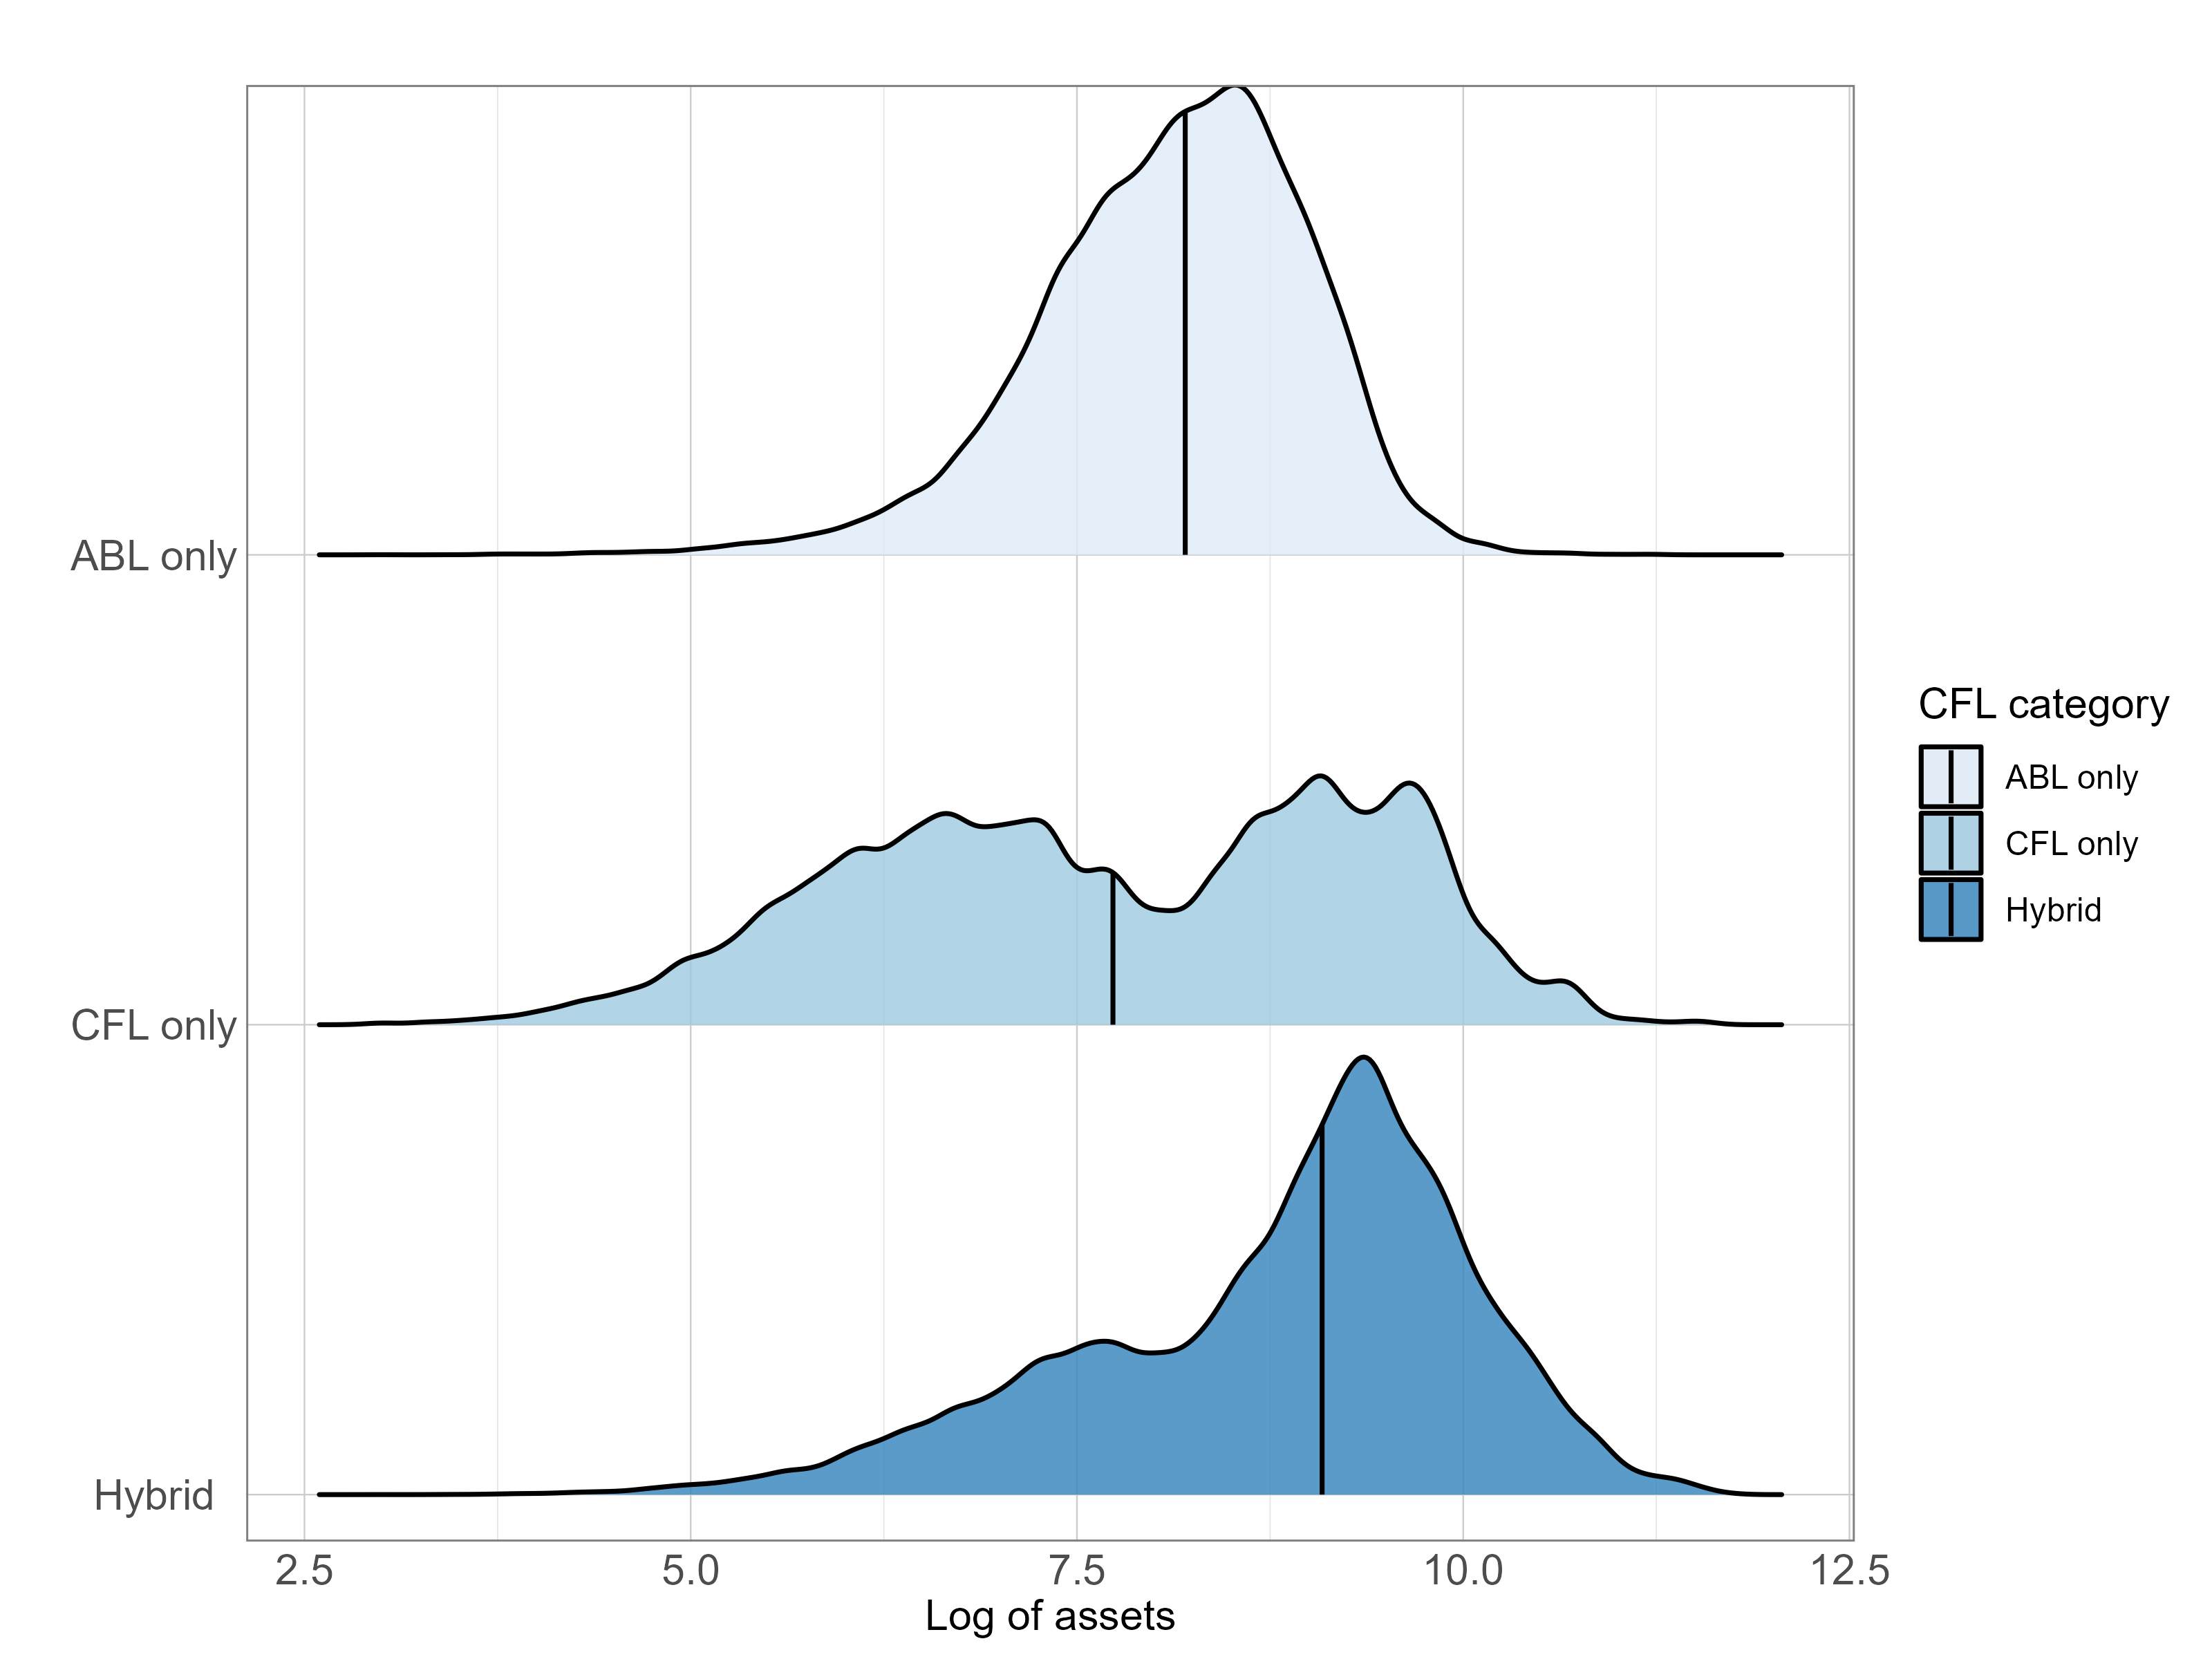
\includegraphics[width=0.9\textwidth]{ridges.png} 
    
     \small The distribution of assets size by categories of CFL reliance. The vertical lines represent median values. 
\end{figure}

\noindent In line with the previous findings of Lian and Ma (2021) and Öztürk (2022), the total outstanding debt volume that can be classified as CF-based is relatively stable around 75\%. However, starting from 2019, this share drops significantly - from 79\% in 2018Q4 to 71\% 2019Q4 - and it does not fully recover until the end of the sample. It is not clear what causes this abrupt shift in aggregate CFL reliance. Unfortunately, I cannot compare with previous studies because they do not investigate this time period. One explanation could be the Covid-induced economic crisis. However, this leaves the initial drop. which happen before the pandemic had a substantial impact on North American economies unexplained. 

\begin{figure}[H]  % [h] indicates placing the image here
    \centering
    \caption{The share of cash flow-based debt to total debt} \label{chart:CFLshare}
    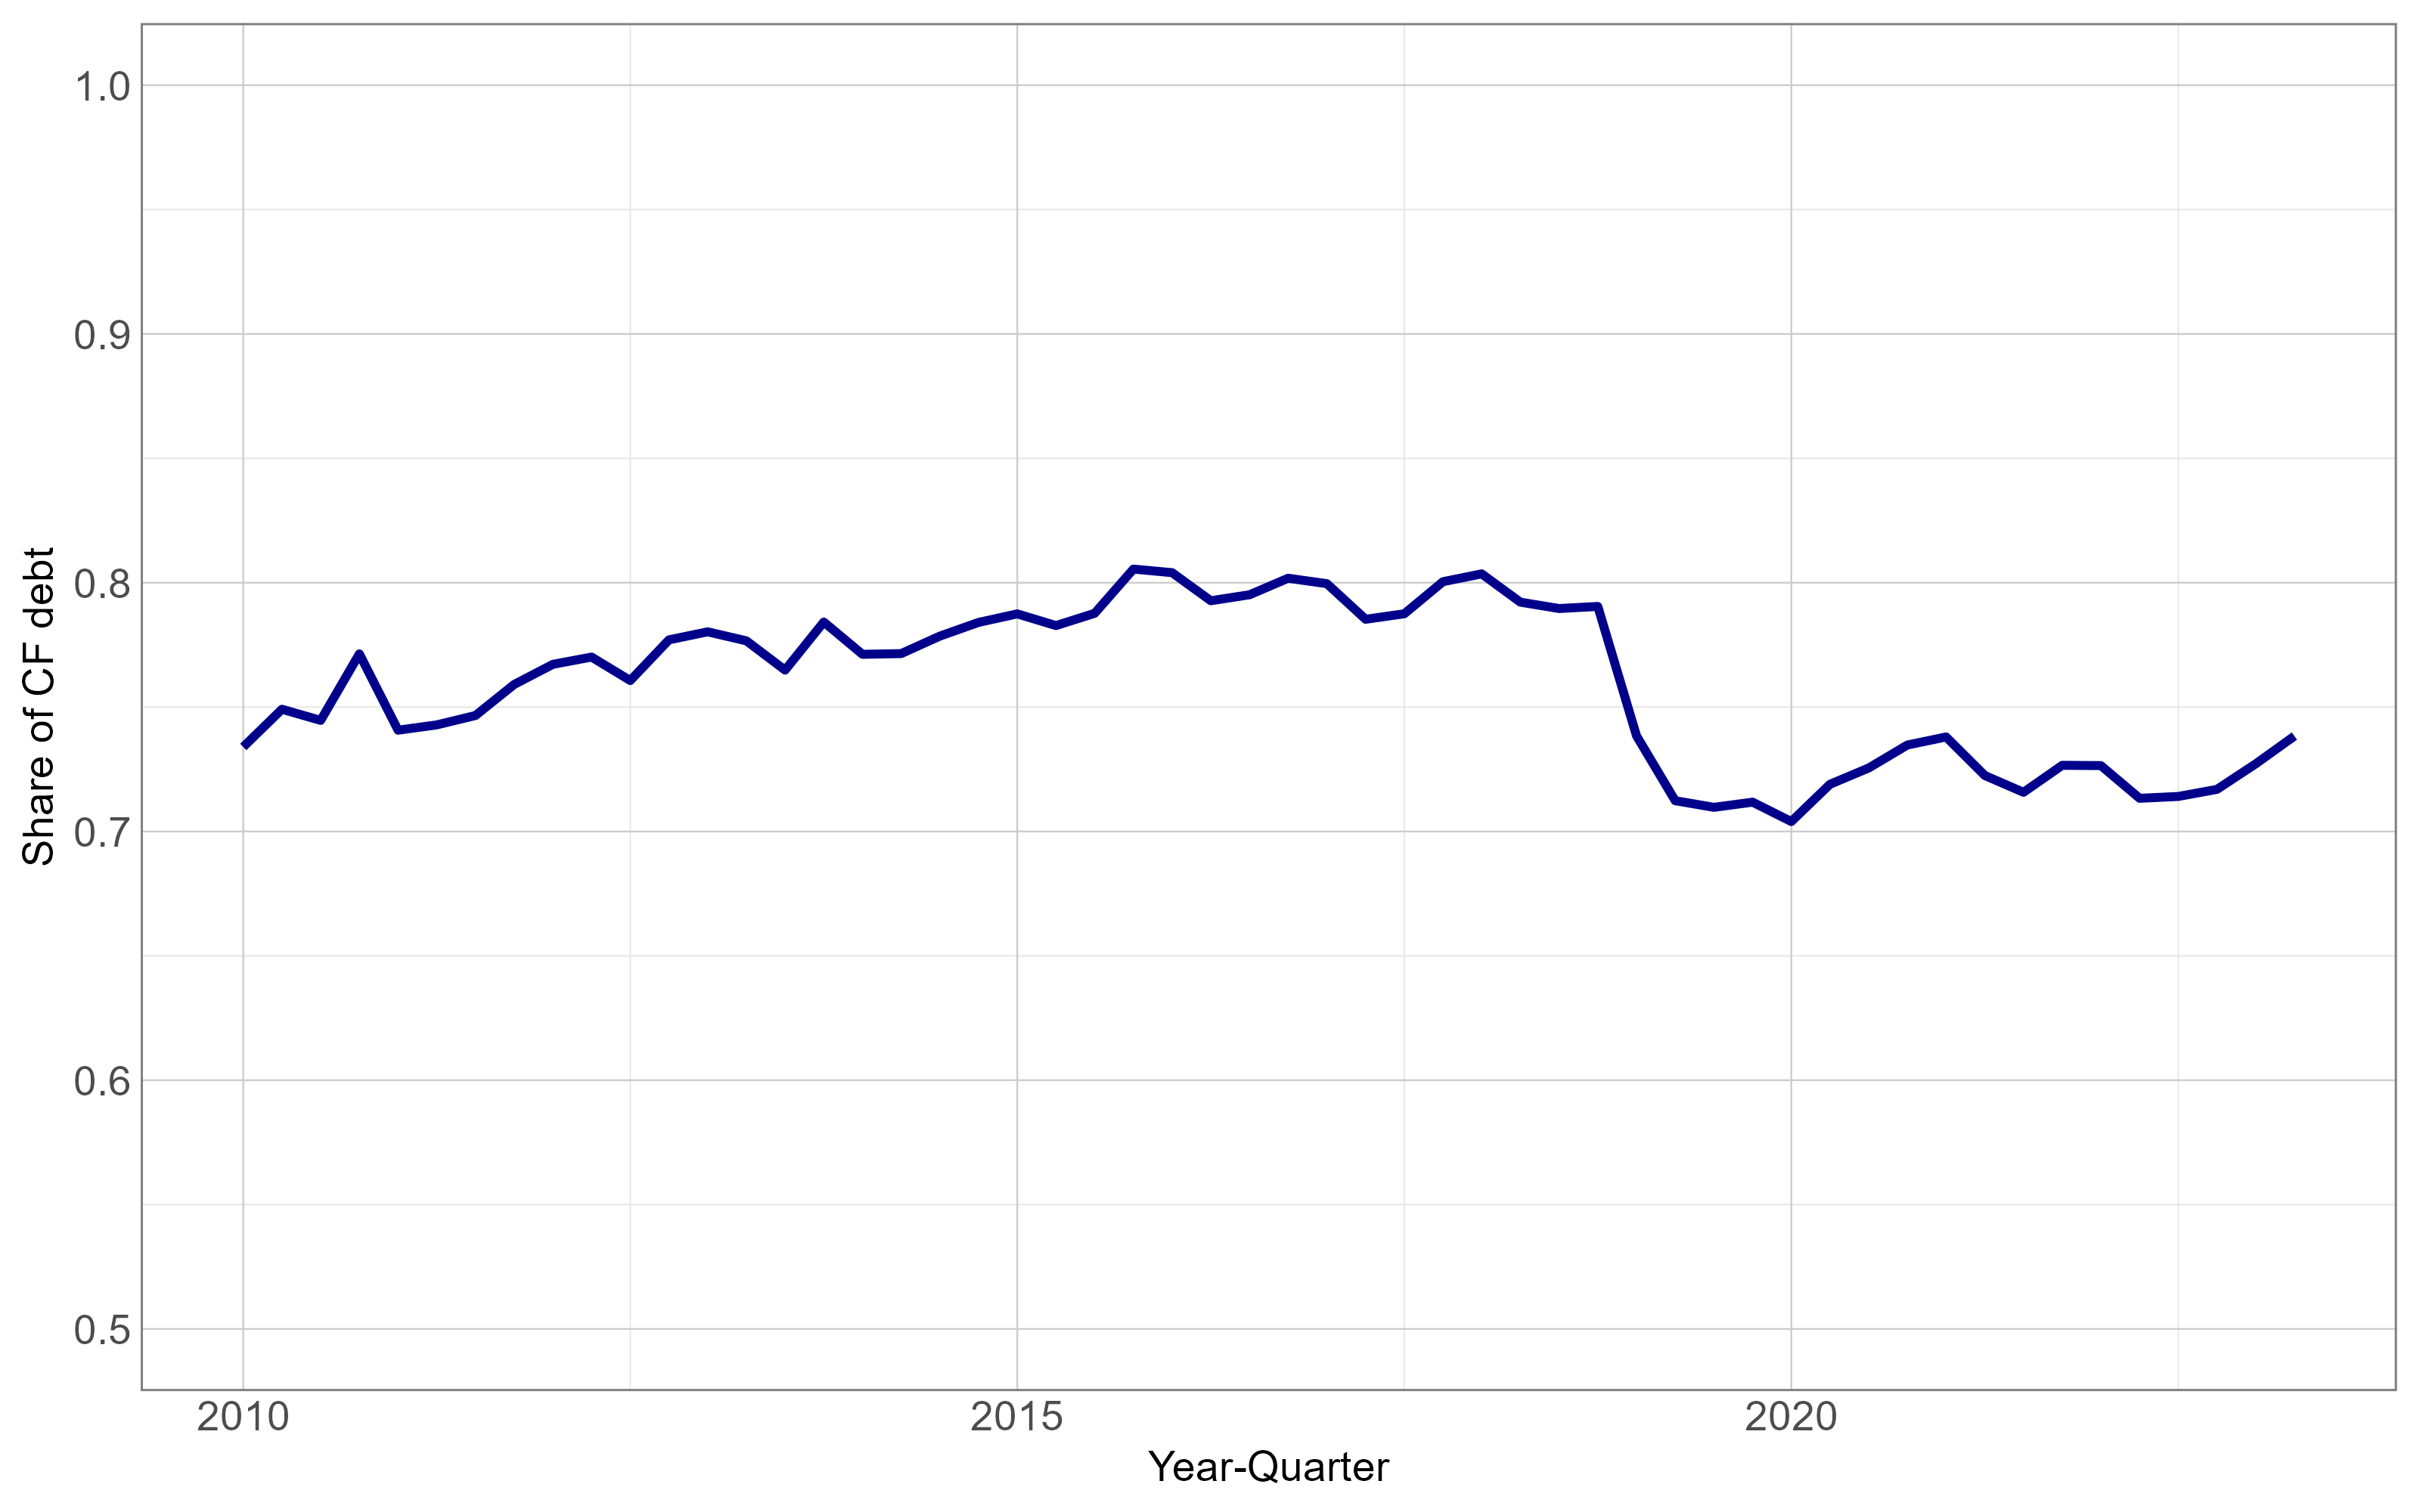
\includegraphics[width=0.8\textwidth]{CFshare.png}
    
     \small The share CFL debt to total debt, by volume between 2010Q1 and 2023Q3
\end{figure}

\noindent Figure 2. of appendix shows the share entries (red) and exits (blue) from the CFL debt market. Plotted against firm age, these show a steadily decreasing trend. Some of this might simply be down to the fact that once a firm entered the CFL market, it would first have to exit to be able to enter again. This seems relatively unlikely even though there is some churning on the extensive margin. Plotted against size, firms are most likely to enter around 1-10 million of total assets and most likely to exit at a size of 10-100 million of total assets. This is consistent with the U-shaped CFL reliance (figure 1.), which indicates that firms of this size rely on CF-based borrowing to a lesser extent. 

\begin{figure}[H]  % [h] indicates placing the image here
    \centering
    \caption{The share firms exiting and entering the CFL market}\label{chart:exitenter}
    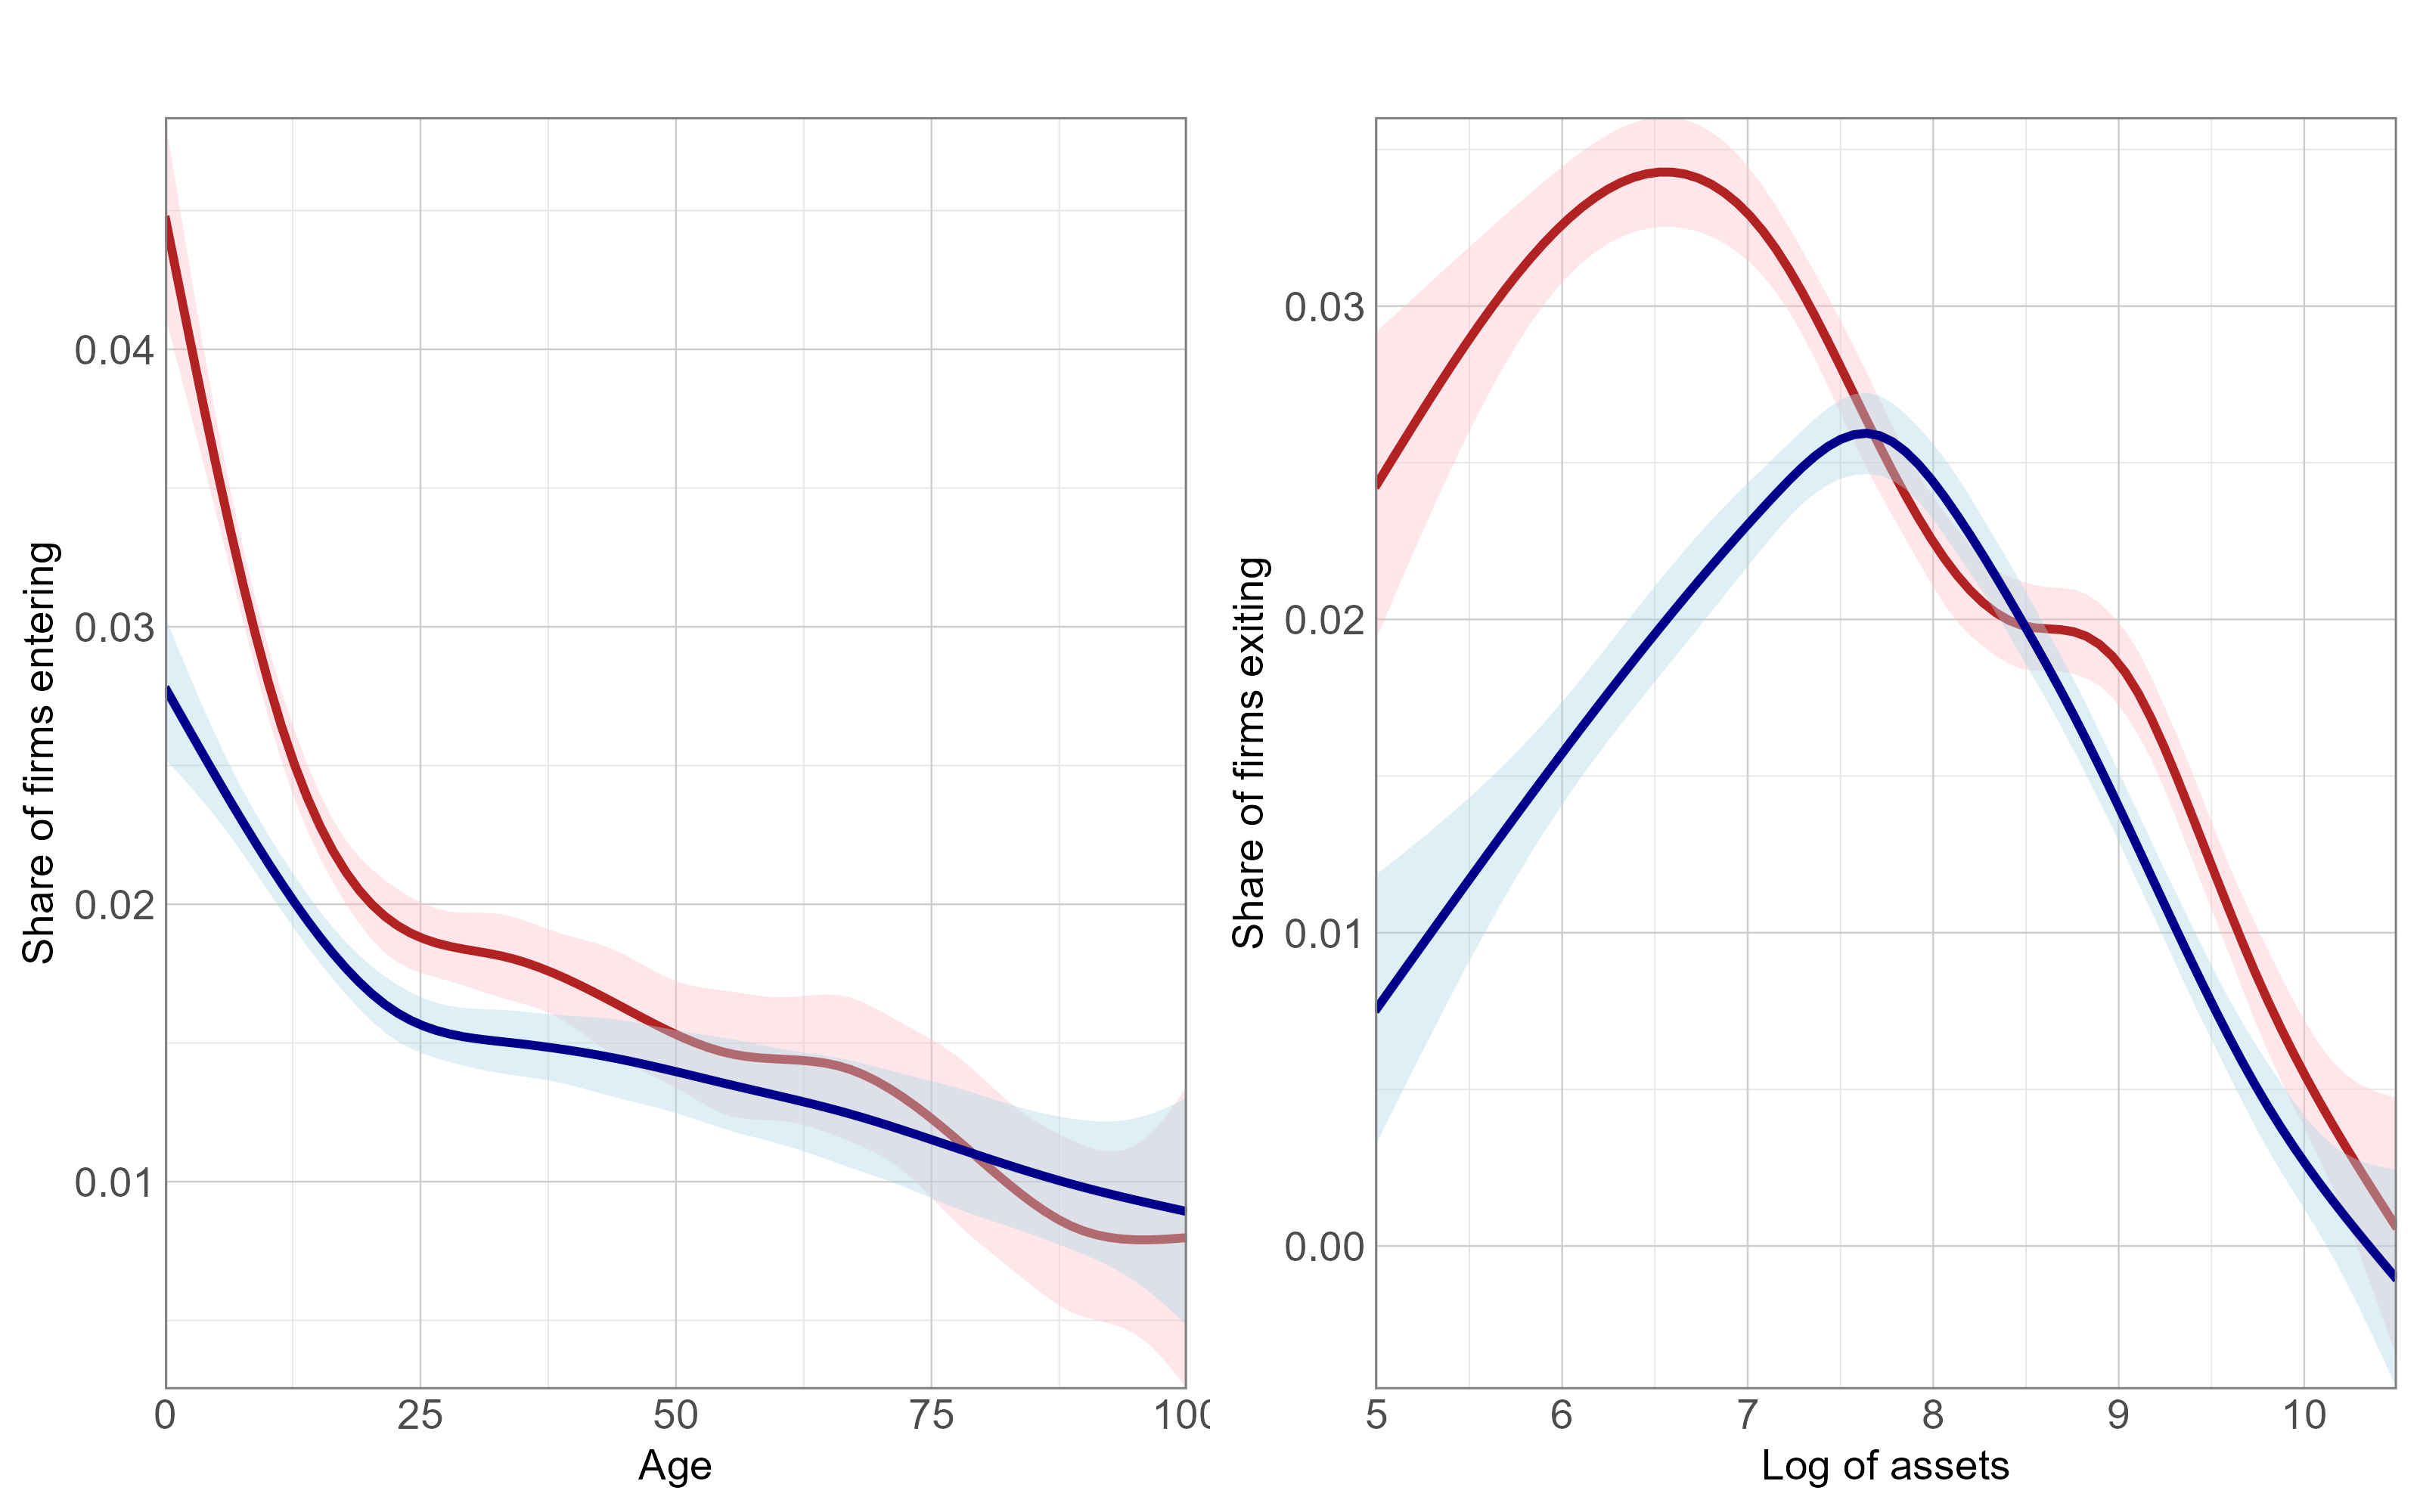
\includegraphics[width=0.8\textwidth]{exit_entry.png} 
    
     \small Moving average of the probability of entering and exiting the CF-based debt market. The blue line indicates exits, whereas the red line shows entries.
\end{figure}

\noindent Figure 3. shows a moving average of CFL reliance as a function  of different explanatory variables. Plotting this variable against revenue and the number of employees yields the same U-shape as in the case of assets. However, revenue and employees become insignificant in the multivariate analysis, once assets are taken into account. Hence, I focus on total assets in the main body of the analysis. Similarly to the multivariate analysis, leverage seems to be an important determinant of CFL reliance: the the least indebted firms, the average is close to 25\% which increases to around 75\% for the most indebted firms. Conversely, pledgeability, which is an important determinant in the multivariate analysis, does not exhibit a visible, strong correlation with cash flow-based lending (CFL) reliance. On interesting observation that firms which realize large losses compared to their size tend be cash-flow based borrowers. This might help explaining why there is a negative association in the multivariate analysis between the two variables. Finally, in-line with the pooled OLS regression results, firm age is also positively correlated with CFL-reliance.

\begin{figure}[H]  % [h] indicates placing the image here
    \centering
    \caption{CFL reliance in relation to the regression variables} \label{chart:CFL}
    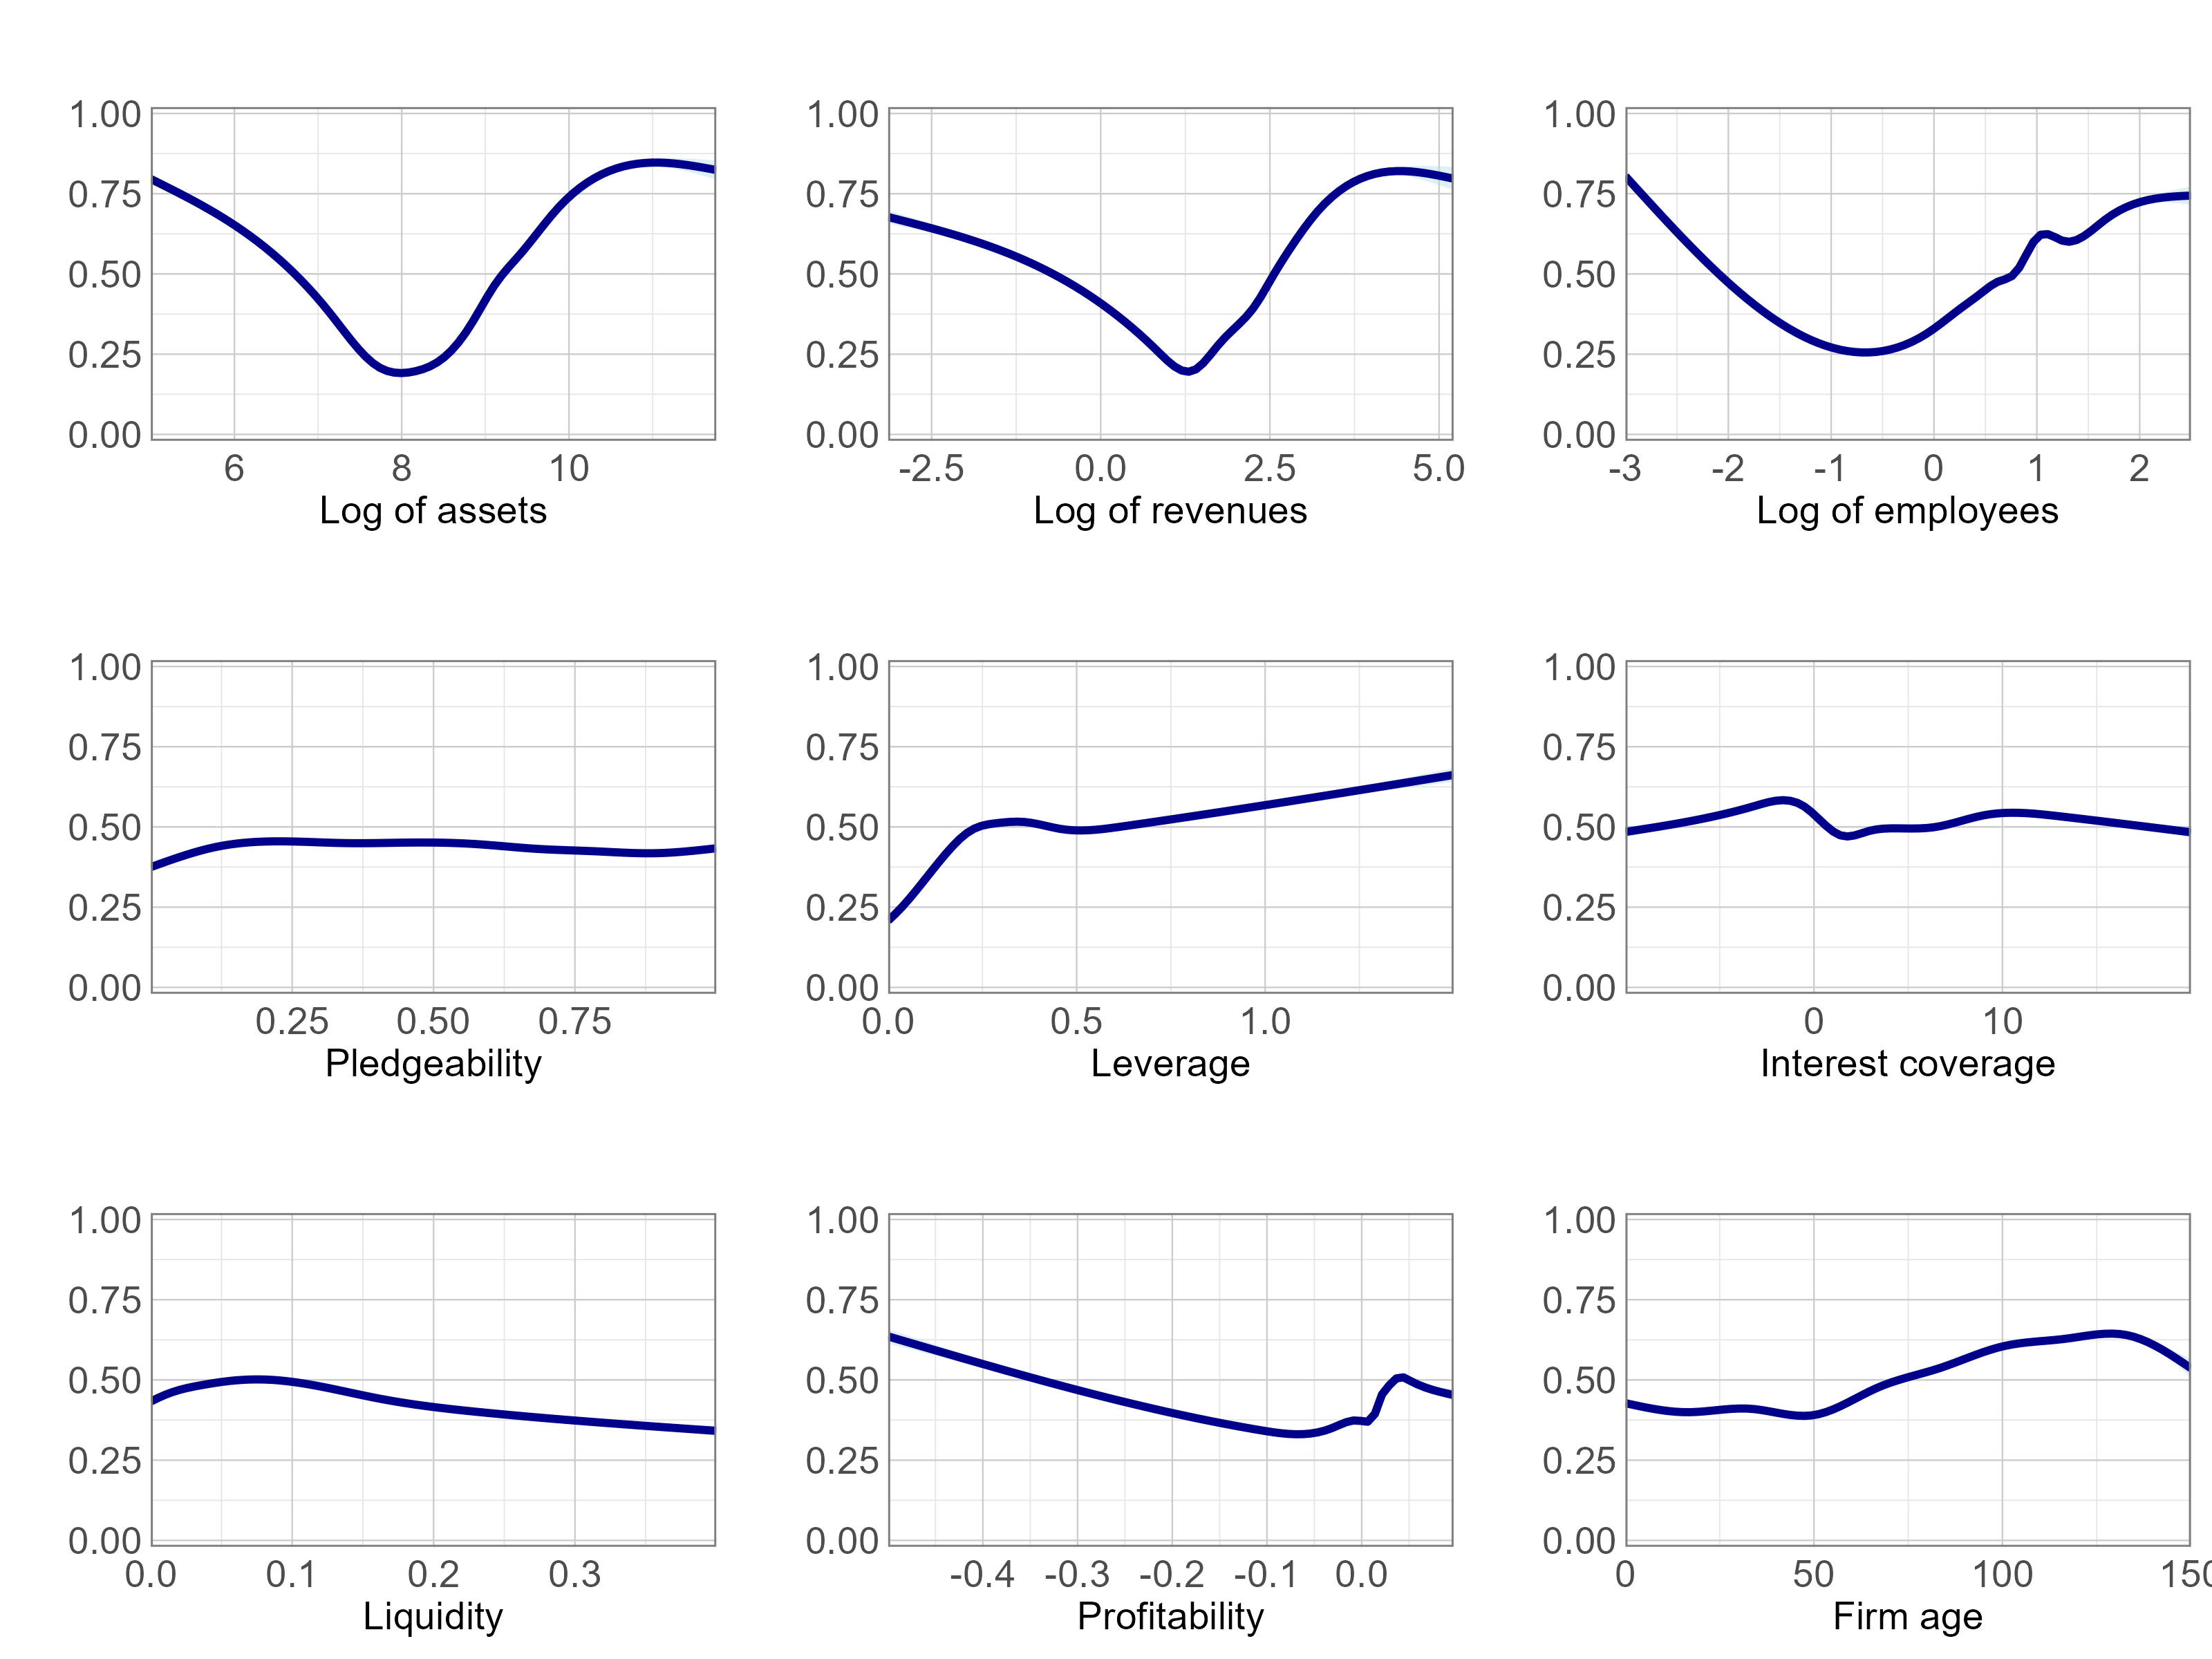
\includegraphics[width=1\textwidth]{varCFL.png}
     \small Moving average of CFL reliance in relation to other regression variables.
\end{figure}

\newpage

\subsubsection{Orbis and Capital IQ evidence}

In the following, I present results from the combination of Orbis and capital IQ data.\footnote{I discuss connecting these datasets in section \ref{sec:A3}.} Orbis contains a wide range of traded and non-traded companies as well. However, I only have detailed debt information on firms that are included in Capital IQ, which mostly focuses on traded firms. Additionally, due to the absence of a common unique firm identifier, matching these two datasets is not perfect. Hence, this dataset is not representative of the entire population of firms in these countries. Nonetheless, it could offer valuable insights into the impacts of legal and institutional frameworks on CF-based lending, given the limited availability of cross-country evidence in existing literature. \vspace{3mm} \\
Although both CapitalIQ and Orbis contains observations from every major economy, I only discuss countries that provide a sufficient number of good quality matches. Therefore, in figure 4 and 5, I present evidence from six Asian and two North American economies only. Additionally, I present `Full Sample' results, which comprise all good quality matches across the world. The first thing to discern from figure 4, is that country differences matter. In Japan, which traditionally relies on asset-based debt contracts, the share of firms that only hold asset-based debt is around 70\%. On the other hand, most Taiwanese firms rely on a mix of asset-based and CF-based debt contracts, which means that only around 20\% of the holds a purely asset-based debt portfolio. \vspace{3mm} \\
In general, North American economies have a higher average reliance on CF based borrowing than their Asian counterparts. Lian and Ma argues that using asset based contracts is an issue of tradition in Japan. For other Asian economies, lower reliance is could be down similar reasons or to differences in bankruptcy practices. In figure 5, I test the persistence of the U-shaped CFL reliance across firm sizes: it holds for the US, Canada and India as well as for the full sample. However, no discernible U-shape is observable for most Asian economies (with the exception of South Korea) where CF-based lending is not as prevalent.

\begin{figure}[H]  % [h] indicates placing the image here
    \centering
    \caption{The cumulative distribution function of CFL reliance, across countries} \label{chart:orb1}
    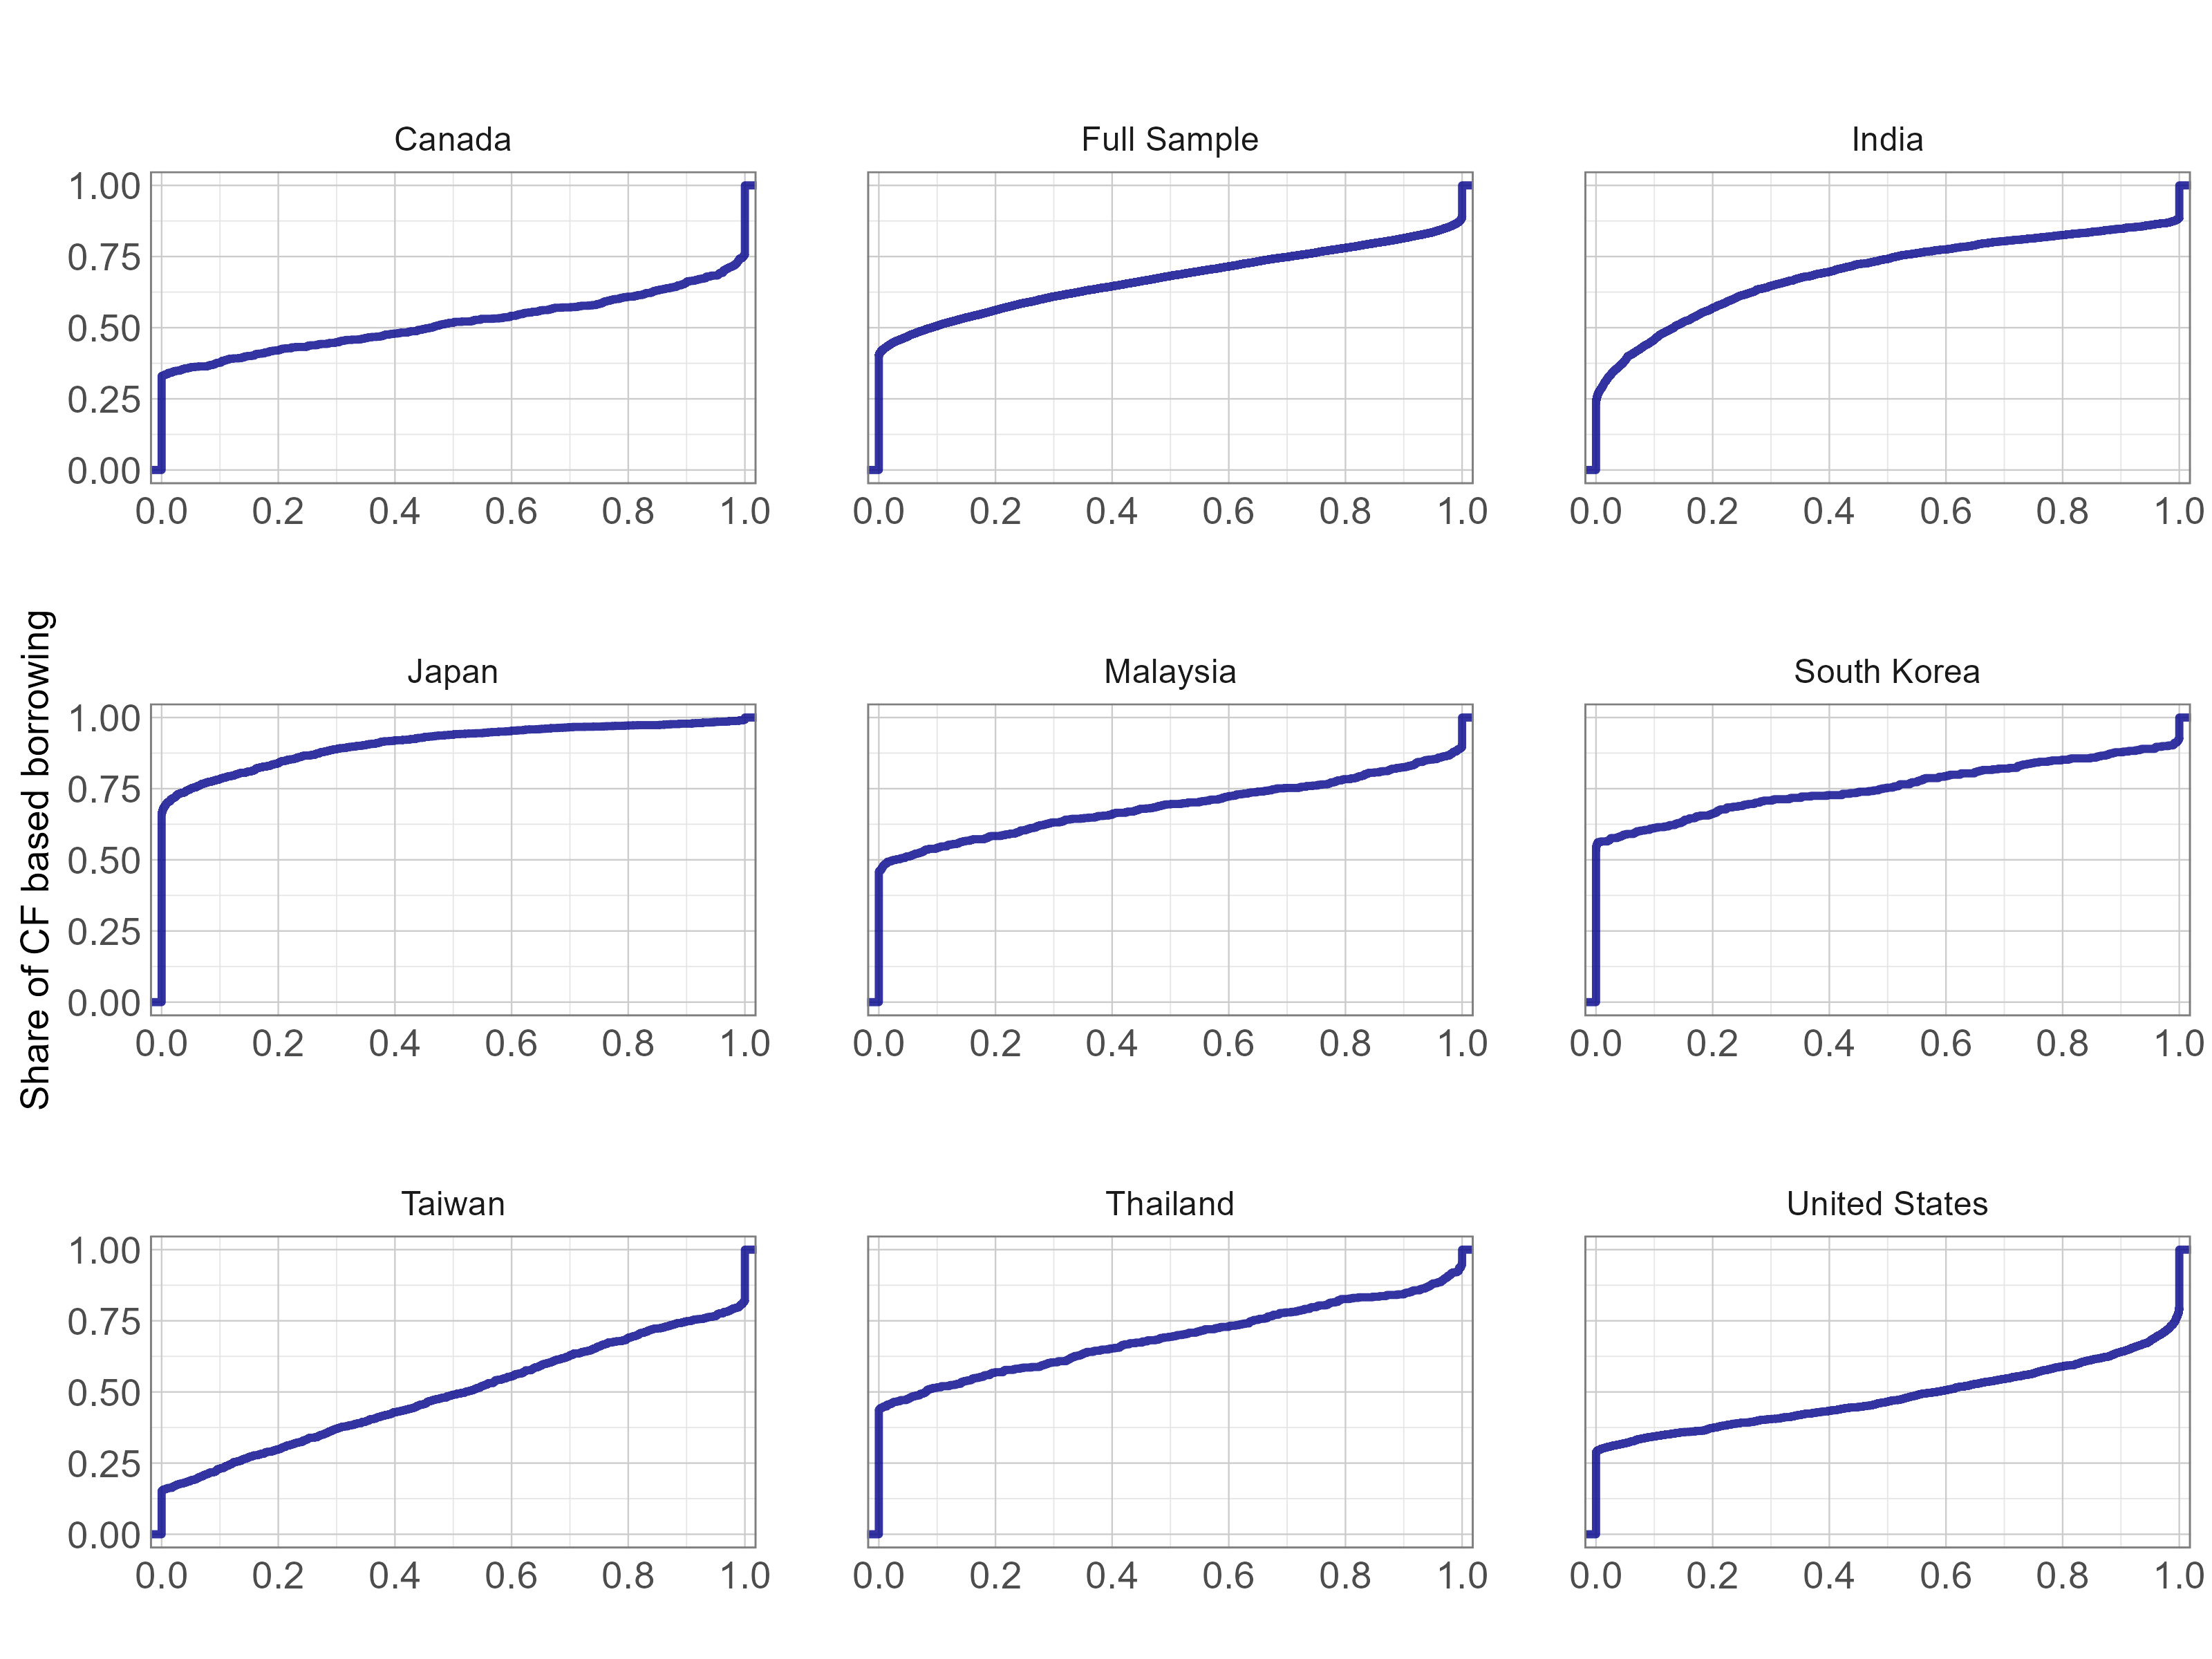
\includegraphics[width=1\textwidth]{cdf_country.png}
    \small The cumulative distribution of CFL reliance in selected economies and in the full sample
\end{figure}

\begin{figure}[H]  % [h] indicates placing the image here
    \centering
    \caption{The distribution of CFL debt over firms size, across countries} \label{chart:orb2}
    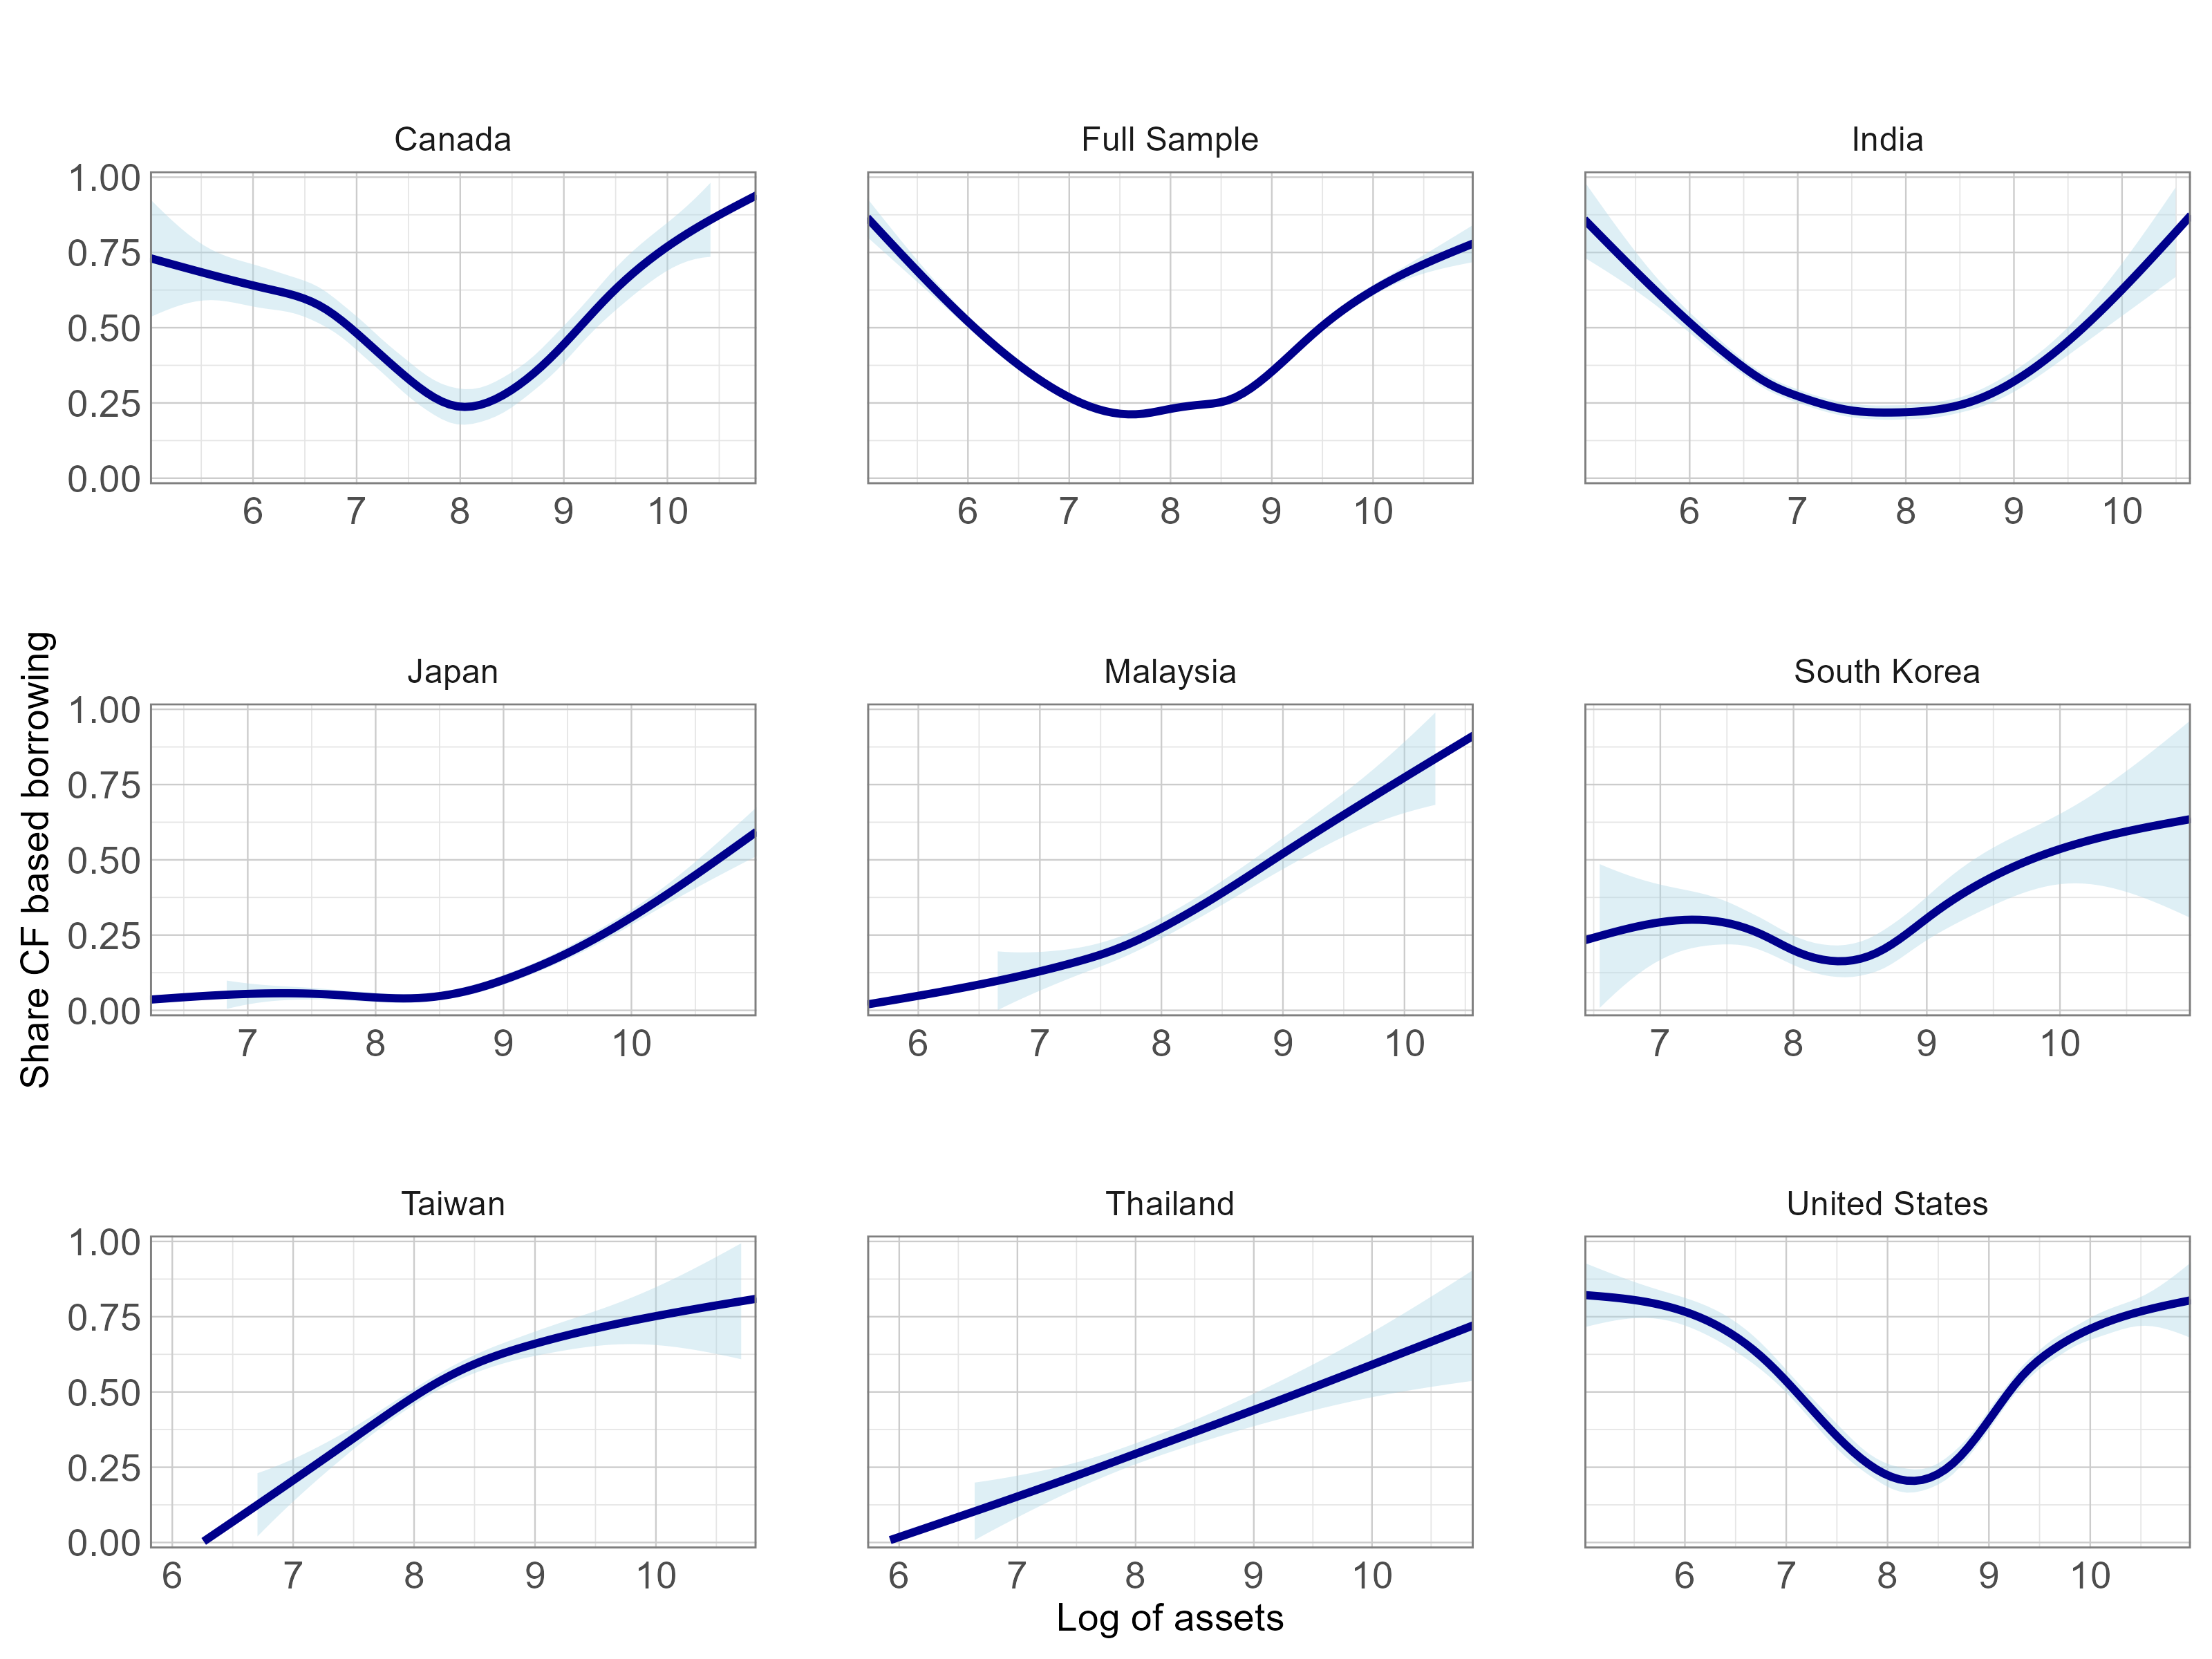
\includegraphics[width=1\textwidth]{smoothy_country.png}
    \small CFL reliance against the logarithm of assets in selected economies and in the full sample
\end{figure}


\end{document}